



\chapter{Ingeniería de Características y Representación de la Data}{\label{Cap4}}



\section{Introducción}



Hasta ahora, hemos asumido que los datos vienen como un    arreglo o una  matriz  bidimensional de números de puntos flotante (floatingpoint), donde cada columna es una característica continua que describe la data de puntos. Para muchas aplicaciones, esto no así  cómo se recopilan los datos.  Un tipo  de característica   particular  muy común son las características categóricas, también conocido como las características discretas, y  por lo general,  son no  numéricos.  La distinción entre las características categóricas y las características continuas es análoga para la distinción entre la clasificación y la regresión, sólo el  aporte de la  entrada más que  la salida. Los ejemplos de características continuas que hemos visto son  brillos de pixeles y las medidas del tamaño en flores Iris, y   ejemplos de características categóricas son la marca de un producto, el color de un producto o  el departamento de ventas (como libros, ropa, hardware, etc.).  Éstas son propiedades que puede describir un producto, pero no varían en forma continua. Un producto que pertenece  al departamento de ropa o al departamento de libros. No hay opción en el medio libros y ropas, y ningún orden natural para las diferentes categorías (los libros no son mayores o menos que la ropa, el hardware no está entre libros y ropas).\\

 Es muy importante considerar la natuarleza de los datos; ya que estos  tendrán un enorme efecto sobre el desempeño del modelo de aprendizaje  automático. En los Capítulos \ref{Cap2}  y \ref{Cap3} vimos que re-escalar de los datos es muy importante; puede suceder que si no se re-escalan los  datos (digamos, con  varianza  unitaria),   puede aparecer alguna diferencia  si representa una medida en centímetros o pulgadas.
 También vimos en el Capítulos \ref{Cap2}  que puede ser útil aumentar la data con características adicionales, como sumar interacciones (los productos) de características o polinomios más general.\\


La técnica que estudia  cómo representar mejor los datos para una aplicación particular es conocida  como Ingeniería de Característica\index{Ingeniería de Característica}, y es una de las principales tareas de científicos de datos y los profesionales  del aprendizaje automático tratando de resolver problemas del mundo real. La representación de los  datos en la forma correcta puede tener una mayor influencia sobre el rendimiento del modelo supervisado más que los parámetros exactos que se puedan seleccionar.\\


En este capítulo, primero abordaremos  el caso importante y muy común de características categóricas, y daremos algunos ejemplos de transformaciones útiles para combinaciones específicas de características y modelos.\\



\section{Variables Categóricas}

Como  ejemplo, usaremos la dataset de Ingresos de Adultos de los Estados Unidos, derivada de la base de datos  censos 1994. La tarea con la  data Ingresos es predecir si un trabajador tiene un ingreso superior o inferior a \$50,000. Las características en esta dataset incluyen la edad del trabajador, tipo de empleo (trabajador por  cuenta propia,  industria privada o empleado del gobierno, etcétera.), educación,  género,  horas de trabajo por la semana, ocupación, y otros. La tabla \ref{Tabla01}  muestra las primeras entradas de la  dataset Ingresos de Adultos.\\



El objetivo en este caso  es expresado como una tarea de clasificación con dos clases para el ingreso,   $<= 50k $  y  $ > 50k$. También se podría  predecir el ingreso exacto, y hacer esta tarea como una regresión.  Sin embargo, eso sería  más difícil, pero por ahora  nuestro interés es  la división del ingreso  para entender.\\

\hspace{-0.6cm} Tabla \ref{Tabla01}. La primeras  entradas de la data  Adultos
\vspace{-0.4cm} 
\begin{figure}[h!]
	%\centering
	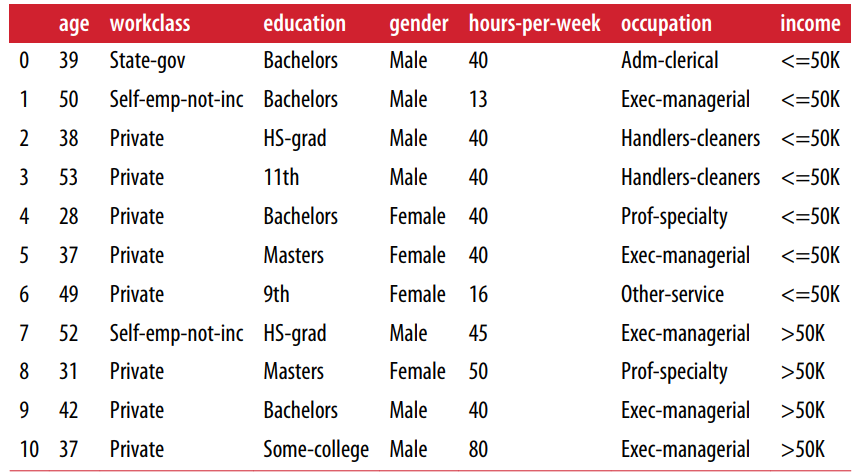
\includegraphics[scale=0.55]{Imagen_Machine/Tabla01}
\end{figure}\label{Tabla01} 

	
En esta data, la edad y las horas por la semana son características continuas, el cuál sabemos como se trata; el tipo de trabajo, educación,  sexo, y la ocupación son características  categóricas, sin embargo, todos ellos vienen de una lista fija de valores posibles, en una distinción de rango que denota una  propiedad cualitativa, en lugar de una cantidad.\\	
	



Como un punto de partida, digamos que queremos que un clasificador de regresión logística  aprenda  en esta data.  Sabemos  del Capítulo \ref{Cap2} que  una regresión logística hace predicciones   $\hat{y}$, mediante la siguiente fórmula:

\[ \hat{y} = w[0] * x[0] + w[1] * x[1] + ... + w[p] * x[p] + b > 0 \]


Donde $w[i]$ y  $b$ son coeficientes aprendidos en el conjunto de entrenamiento,   and $x[i]$ son las entradas de las características.    Esta fórmula tiene sentido cuando $ x[i]$ son números, pero cuando la $X[i]$ no son números no tiene sentido, como en el caso de $x[2]$  es "Masters"{} o "Bachelors".
Claramente necesitamos representar estos datos en alguna otra forma que permita aplicar el modelo regresión logística. 

En la  siguiente sección se explica cómo podemos  tratar este problema.
	
%  https://machinelearningmastery.com/one-hot-encoding-for-categorical-data/

\subsection{Codificación One-Hot  (one-hot-encoding) }	

%  Codificación única (One-Hot-Encoding) o  variables ficticias (Dummy Variables)
 
La forma más común para representar variables categóricas es usando la Codificación One-Hot   o  one-out-of-N\index{one-out-of-N}, también conocido como  variables dummy o variables ficticias. La idea detrás de las  variables dummy es reemplazar una variable categórica con una o más características nuevas que pueden tomar los  valores 0 y 1. Los valores 0 y 1 dan sentido a la fórmula de clasificación binaria lineal (y para todos  modelos en {\ttfamily{scikit-learn}}), y podemos representar  {\bf \emph{cualquier número de  categorías} }   introduciendo una nueva característica  por  categoría, como se describe aquí.\\


Digamos para la característica  workclass  (tipo de empleo)  los valores posibles  "{}Government Employee"{}  (empleado del gobierno) , "{}Private Employee"{}  (empleado privado) , "{}Self Employed"{} (empleado por cuenta propia) , y "{}Self Employed Incorporated"{}   (empleado por cuenta propia calificado).   Para codificar estos cuatro valores posibles, creamos cuatro características nuevas, designadas "{}Government Employee"{}, "{}Private Employee"{}, "{}Self Employed"{}, y "{}Self Employed Incorporated"{}.     
El valor de la nueva característica será  1 si el  tipo de empleo para esta  persona tiene el valor  correspondiente  y  0 en otro caso, así exactamente sólo una de las cuatro características nuevas será igual  1 para cada dato (en este caso la fila).  Por este motivo esta codificación es llamada  one-hot o one-out-of-N\index{codifecaión one-hot}.\\




El principio se ilustra en la Tabla \ref{Tabla02}, donde sólo la característica workclass  es codificada usando  cuatro nuevas características.  Al usar esta data en un algoritmo  machine learning,  descartaríamos la característica original workclass y sólo mantendríamos las nuevas  características con  0–1.  En la tabla  \ref{Tabla02} se codifica la característica workclass usando una codificación one-hot.\\	


\hspace{-0.6cm} Tabla \ref{Tabla02}. Característica workclass codificada con  one-hot
\vspace{-0.4cm} 
\begin{figure}[h!]
	%\centering
	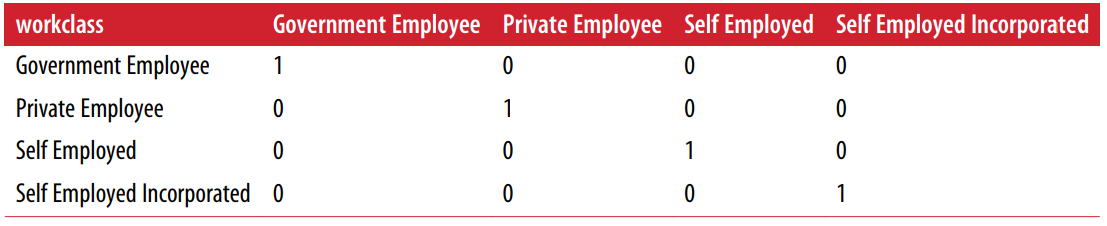
\includegraphics[scale=0.55]{Imagen_Machine/Tabla02}
\end{figure}\label{Tabla02} 

\newpage

\begin{minipage}[t]{0.2\textwidth}
	\centering\raisebox{\dimexpr \topskip-\height}{%
		
\includegraphics[width=\textwidth]{Imagen_Machine/Pajaro.png}}
\end{minipage}%\hfill
\begin{minipage}[t]{0.75\textwidth} 
	{\scriptsize	
	La codificación one-hot que usamos es muy similar, \:  pero no idéntica, a la codificación 
	dummy usada en Estadística. \: Por simplicidad, \: codificamos cada categoría con una característica binaria diferente. En  Estadística, es común  codificar una característica categórica con $k$ valores posibles diferentes en $k$–$1$  características (el último es representado como todos los ceros). Esto se hace  	para simplificar el análisis (técnicamente hablando,  esto evitará hacer que la matriz de datos sea deficiente en rango).}
\end{minipage} \\


Hay dos formas para convertir los datos  con la codificación one-hot a  variables  categóricas, mediante el uso de {\ttfamily pandas}  o  {\ttfamily scikit-learn}.  Al momento de escribir estas notas, el uso de  {\ttfamily pandas}  es un poco más fácil, así que elegimos  esta ruta. Primero cargamos la data usando {\ttfamily pandas} como un archivo de valores separados por comas  (CSV):

\begin{lstlisting}  	

In[2]:

   import pandas as pd
   # The file has no headers naming the columns, so we pass header=None
   # and provide the column names explicitly in "names"
   data = pd.read_csv("https://archive.ics.uci.edu/ml/
                       machine-learning-databases/adult/adult.data", 
                       header=None, index_col=False, 
                       names=['age', 'workclass', 'fnlwgt','education',
                              'education-num','marital-status', 'occupation',
                              'relationship', 'race', 'gender', 'capital-gain', 
                              'capital-loss', 'hours-per-week', 'native-country',
                              'income'])
   # For illustration purposes, we only select some of the columns
   data = data[['age', 'workclass', 'education', 'gender', 'hours-per-week',
                'occupation', 'income']]
   # IPython.display allows nice output formatting within the Jupyter notebook
   display(data.head())
   
\end{lstlisting}   


\hspace{-0.6cm} Tabla \ref{Tabla03}. Las primeras cinco filas de la data Adultos
\vspace{-0.4cm} 
\begin{figure}[h!]
	%\centering
	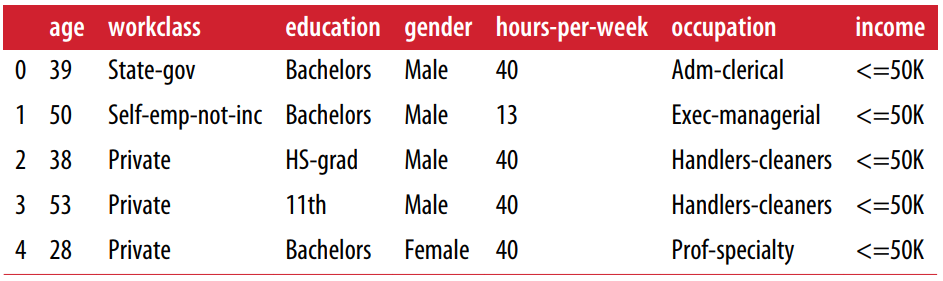
\includegraphics[scale=0.55]{Imagen_Machine/Tabla03}
\end{figure}\label{Tabla03} 
\newpage

\subsection{Verificación  de datos categóricos codificados en  cadena de caracteres (string)}
%  Checking string-encoded categorical data


Después de leer un conjunto de datos como este,  es buena práctica  comprobar primero si una columna contiene datos categóricos significativos. Cuando se trabaja con datos que fueron introducidos por seres humanos (por ejemplo, usuarios en un sitio web), podría no haber un conjunto fijo de categorías, y differencias en la ortografía y la capitalización podrían requerir preprocesamiento. Por ejemplo, podría ser que algunas personas especificaran el género como  "{}masculino"{} y  otras como "hombre"{},  y 
podríamos  querer representar estas dos entradas usando la misma categoría.   Una buena manera de comprobar el contenido de una columna es usando la función {\ttfamily value\_counts }  de una serie de pandas (el tipo de una sola columna en un DataFrame), para mostrarnos cuáles son los valores únicos y con qué frecuencia aparecen:

\begin{lstlisting}  

In[3]: print(data.gender.value_counts())

Out[3]:

   Male 21790
   Female 10771
   Name: gender, dtype: int64
  
\end{lstlisting} 

Podemos ver que hay exactamente dos valores para el género en este conjunto de datos, masculino y femenino, lo que significa que los datos ya están en un buen formato para ser representados utilizando la codificación One-Hot.  En una aplicación real, debe observar todas las columnas y verificar sus valores. En este caso lo vamos a omitir  por la brevedad.

 Hay una manera muy sencilla de codificar los datos en  {\ttfamily pandas}, usando la función {\ttfamily get\_dummies}, esta función  transforma automáticamente todas las columnas que tienen un tipo de objeto (como cadenas) o  categóricas (un concepto especial de {\ttfamily pandas} del que aún no hemos hablado):\\


\begin{lstlisting}%[frame=single]

In[4]:

   print("Original features:\n", list(data.columns), "\n")
   data_dummies = pd.get_dummies(data)
   print("Features after get_dummies:\n", list(data_dummies.columns))

Out[4]:

    Original features:
    ['age', 'workclass', 'education', 'gender', 'hours-per-week',
     'occupation', 'income']

   Features after get_dummies:
    ['age', 'hours-per-week', 'workclass_ ?', 'workclass_ Federal-gov',
     'workclass_ Local-gov', 'workclass_ Never-worked', 'workclass_ Private',
     'workclass_ Self-emp-inc', 'workclass_ Self-emp-not-inc',
     'workclass_ State-gov', 'workclass_ Without-pay', 'education_ 10th',
     'education_ 11th', 'education_ 12th', 'education_ 1st-4th',
      ...
     'education_ Preschool', 'education_ Prof-school', 
     'education_ Some-college','gender_ Female', 'gender_ Male', 
     'occupation_ ?', 'occupation_ Adm-clerical', 
     'occupation_ Armed-Forces', 'occupation_ Craft-repair',
     'occupation_ Exec-managerial', 'occupation_ Farming-fishing',
     'occupation_ Handlers-cleaners',
      ...
     'occupation_ Tech-support', 'occupation_ Transport-moving',
      'income_ <=50K', 'income_ >50K']

\end{lstlisting}


Puede ver que las características continuas edad y horas por semana no presentan cambios, mientras que las características categóricas se ampliaron en una nueva característica para cada valor posible 
(por categoría):

\begin{lstlisting}

In[5]:

   data_dummies.head()

Out[5]:

\end{lstlisting}

\hspace{-0.6cm} Tabla \ref{Tabla04}. Las primeras cinco filas de la data Ingresos
\vspace{-0.4cm} 
\begin{figure}[h!]
	%\centering
	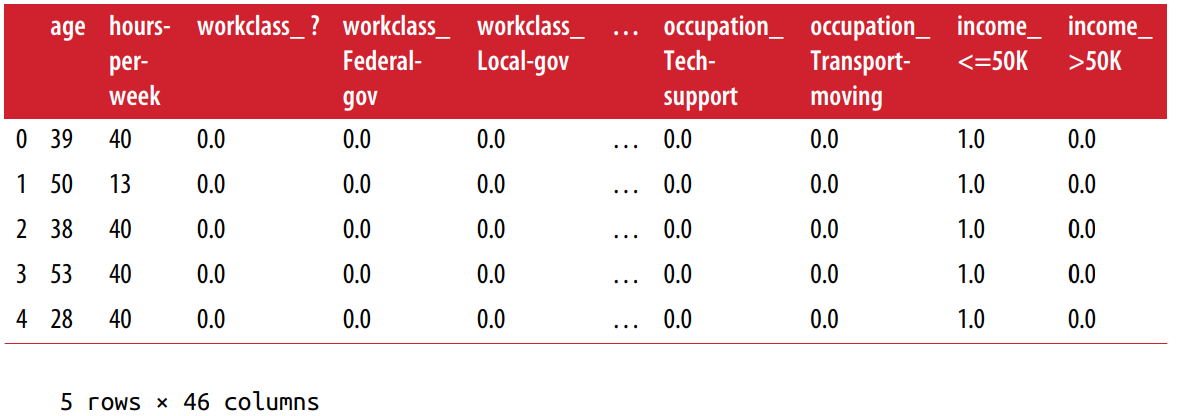
\includegraphics[scale=0.55]{Imagen_Machine/Tabla04}
\end{figure}\label{Tabla04} 

Ahora podemos usar el atributo {\ttfamily values}  para convertir la  {\ttfamily  DataFrame  data\_dummies  } en un arreglo  {\ttfamily  NumPy}  (matriz), y luego entrenar un modelo de aprendizaje automático sobre esa data. Debe tener cuidado al separar la variable  objetivo de los datos antes de entrenar un modelo (pues ahora está codificada en dos columnas de ingresos).    Incluyendo la variable  salida, o alguna propiedad derivada de la variable  salida, en la representación de características es un error muy común en la construcción de modelos de aprendizaje automático supervisado.


\begin{minipage}[t]{0.2\textwidth}
	\centering\raisebox{\dimexpr \topskip-\height}{%
		
\includegraphics[width=\textwidth]{Imagen_Machine/Escorpion}}
\end{minipage}%\hfill
\begin{minipage}[t]{0.75\textwidth} 
	{\scriptsize		
		Tenga cuidado: la indexación de columnas en pandas incluye el final del rango, así que  "{}age"{}:  "{}occupation\_ Transport-moving"{}   incluya  a   "{}occupation\_  Transport-moving"{}. Esto es diferente de dividir  un {\ttfamily array NumPy}, donde el final de un rango no se incluye: por ejemplo,  {\ttfamily  np.arange(11)[0:10] }  no incluye la entrada con el índice 10.\\}
\end{minipage}
\\

En este caso, extraemos sólo las columnas que contienen características, es decir, todas las columnas de  {\ttfamily age } a   {\ttfamily occupation\_  Transport-moving}. Este rango contiene todas las características pero no el objetivo:

\begin{lstlisting}
In[6]:

   features = data_dummies.ix[:, 'age':'occupation_ Transport-moving']
   # Extract NumPy arrays
   X = features.values
   y = data_dummies['income_ >50K'].values
   print("X.shape: {} y.shape: {}".format(X.shape, y.shape))

Out[6]:

    X.shape: (32561, 44) y.shape: (32561,)
    
\end{lstlisting}

Ahora los datos se representan de una manera que el {\ttfamily scikit-learn} puede trabajar,  y podemos proceder como de costumbre:

\begin{lstlisting}
In[7]:

   from sklearn.linear_model import LogisticRegression
   from sklearn.model_selection import train_test_split
   X_train, X_test, y_train, y_test = train_test_split(X, y, random_state=0)
   logreg = LogisticRegression()
   logreg.fit(X_train, y_train)
   print("Test score: {:.2f}".format(logreg.score(X_test, y_test)))

Out[7]:
   
   Test score: 0.81
\end{lstlisting}



\newpage



\begin{minipage}[t]{0.2\textwidth}
	\centering\raisebox{\dimexpr \topskip-\height}{%
		
\includegraphics[width=\textwidth]{Imagen_Machine/Escorpion}}
	%	\captionof{figure}{Caption for fig 1}
	%	\label{fig1}
	%	\includegraphics[width=\textwidth]{example-image-b}
	%	\captionof{figure}{Caption for fig 2}
	%	\label{fig2}
\end{minipage}\hfill
\begin{minipage}[t]{0.75\textwidth} 
	{\scriptsize
		En este ejemplo, ejecutamos  a {\ttfamily get\_dummies} sobre la DataFrame que contiene
		tanto la data de  entrenamiento como la de prueba. Esto es importante para asegurar que
		los valores de las categorías se representan de la misma forma tanto en el conjunto de
		entrenamiento y como en el de prueba.\\		
		Imagine que tenemos la data  entrenamiento y prueba en dos dataframes diferentes.  Si el valor 
		"{}Private Employee"{}   para la característica  workclass no aparece en la data de prueba, {\ttfamily pandas} asumirán que sólo hay tres valores posibles para esta característica y creará solo tres nuevas características ficticias (dummy).  				
		Ahora la data de entrenamiento y prueba tienen diferentes número de características, y no podemos aplicar el modelo que aprendido en la data de entrenamiento al  prueba. Peor aún, imagina la característica  workclass  tiene los valores  "{}Government Employee"{} y "{}Private Employee"{}  en el conjunto de entranamiento, y  "Self Employed"{}  y  "{}Self Employed Incorporated"{}   en el conjunto de prueba.
		En ambos casos, {\ttfamily pandas} crearán dos nuevas características ficticias, por lo que los datos codificados en la dataframe  tendrán el  mismo número de caracteísticas. Sin embargo, las  características ficticias tienen significados completamente diferentes en la data de entrenamiento y en la de  prueba. La columna que significa  "{}Government Employee"{}  para el conjunto de entrenamiento codificaría  "{}Self Employed"{}  para el conjunto de prueba.	\\ 
	 Si construimos un modelo de aprendizaje automático sobre estos datos, funcionaría muy mal, 
	 porque supondría que las columnas significan la misma cosa   (porque están en la misma posición) cuando en realidad tienen significados muy diferentes.  Para solucionar esto, se ejecuta a {\ttfamily get\_dummies} en una DataFrame que contiene los  puntos de datos de entrenamiento y prueba, o asegúrese de que los nombres de las columnas sean los mismos para la data de entrenamiento y prueba, después de  ejecutar  {\ttfamily get\_dummies}, para segurarse de que tengan el misma semántica.}\\
	\end{minipage}




\subsection{Números que se pueden codificar como categorías}
% Numbers Can Encode Categoricals


En el ejemplo de la data  Adultos, las variables categóricas se codificaron como cadenas.
Por un lado, eso abre la posibilidad de errores ortográficos, y además, marca claramente una variable  categórica.   Genearlmente las variables categóricas son codificadas como enteros,  ya sea por facilidad de almacenamiento o debido a la forma en que se recopilan los datos.  Por ejemplo, imagine que los datos del censo en la data  Adultos se recopilaron mediante una pregunta y las respuestas para la clase de trabajo se registraron como 0 (primer casilla etiquetada), 1 (segunda  casilla etiquetada), 2 (casilla marcada tercera), y así sucesivamente. 
Ahora la columna contendrá números del 0 al 8, en lugar de cadenas como  "{}Private"{}, y no será inmediatamente  obvio para alguien que vea la tabla  representada el en conjunto de datos, identificar si se  trata una  variable como continua o categórica.   Sin embargo,   conociendo  que los números indican el estado laboral,  queda claro que estos son estados muy distintos y  no deben ser modelado por una  variable continua. \\




\begin{minipage}[t]{0.2\textwidth}
	\centering\raisebox{\dimexpr \topskip-\height}{%
		
\includegraphics[width=\textwidth]{Imagen_Machine/Escorpion}}
	%	\captionof{figure}{Caption for fig 1}
	%	\label{fig1}
	%	\includegraphics[width=\textwidth]{example-image-b}
	%	\captionof{figure}{Caption for fig 2}
	%	\label{fig2}
\end{minipage}\hfill
\begin{minipage}[t]{0.75\textwidth} 
	{\scriptsize	
	Las características categóricas generalmente se codifican con números enteros. 	El hecho que  sean números no significa que deban ser tratados necesariamente como características continuas.  No siempre está claro si una característica de número entero debe ser tratada como continua o discreta.
	Si no hay un  orden entre la semántica que se codifica (como en el ejemplo de clase de trabajo), la característica debe ser tratado como discreta. 	 Para otros casos, la mejor codificación depende de la tarea particular,   la  data y de qué tipo de algoritmo de aprendizaje automático se utiliza.\\}
\end{minipage}\\


La función {\ttfamily get\_dummies} en {\ttfamily pandas} trata todos los números como continuos 
y no creará variables dummy para ellos. Para evitar esto, puede hacer uso de  {\ttfamily OneHotEncoder} 
de  {\ttfamily  scikit-learn}, para el cual puede especificar cuales  variables son continuas y 
cuáles son discretas, o convertir columnas numéricas en Dataframe de cadenas (strings). Para ilustrar este proceso vamos a crear un objeto tipo DataFrame con dos columnas, una con  cadenas y la  otra con h enteros:

\begin{lstlisting}
In[8]:

   # create a DataFrame with an integer feature and a categorical string 
   # feature
   demo_df = pd.DataFrame({'Integer Feature': [0, 1, 2, 1],
                           'Categorical Feature': ['socks', 'fox', 
                                                   'socks', 'box']})
   display(demo_df)

\end{lstlisting}


\noindent El resultado se muestra en la tabla \ref{Tabla05}.
%\vspace{-0.2cm}
\begin{table}[!h]
	\hspace{0.1cm} \vspace{-0.1cm}	\caption{DataFrame que contiene dos características  categórica, una  string    y la otra con enteros}	
	\label{Tabla05}	
	\hspace{-0.4cm} \begin{tabular}{  l  }
		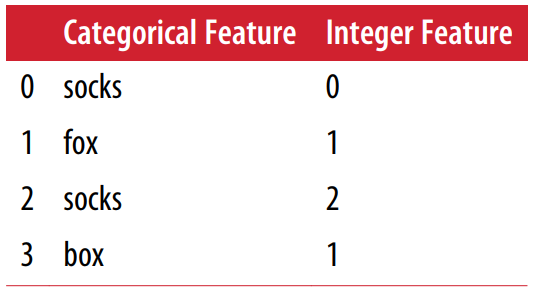
\includegraphics[scale=0.45]{Imagen_Machine/Tabla05}
	\end{tabular}
\end{table}




Usando {\ttfamily get\_dummies} sólo codificará la característica  string y no cambiará la característica de enteros, como puedes ver en la Tabla \ref{Tabla61}.


\begin{lstlisting}%[frame=single]

In[9]:
   
   pd.get_dummies(demo_df)


\end{lstlisting}
%\vspace{-0.5cm}
\begin{table}[!h]
	\hspace{0.1cm} \vspace{-0.1cm}	\caption{Una versión de codificación One-hot  de los datos de la Tabla \ref{Tabla05}, dejando la característica de entero  sin cambiar}	
	\label{Tabla61}	
\hspace{-0.4cm}	\begin{tabular}{  l  }
		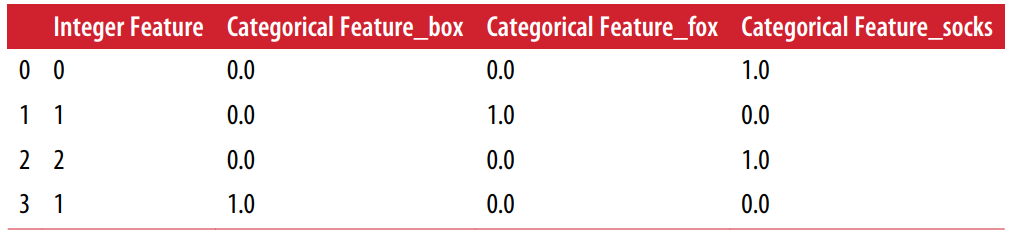
\includegraphics[scale=0.55]{Imagen_Machine/Tabla61}
	\end{tabular}
\end{table}

Si desea que se creen variables   dummy (ficticias) para la columna "{}característica entera"{}, puede enumerar explícitamente las columnas que desea codificar utilizando el parámetro columnas. A continuación, ambas características se considerarán categóricas (véase en la Tabla \ref{Tabla71}): 
	
	\begin{lstlisting}%[frame=single]
	
In[10]:

   demo_df['Integer Feature'] = demo_df['Integer Feature'].astype(str)
   pd.get_dummies(demo_df, columns=['Integer Feature', 
                                    'Categorical Feature'])
		
	\end{lstlisting}
\vspace{-0.9cm}	
\begin{table}[!h]
	\hspace{0.1cm} \vspace{-0.1cm}	\caption{Codificación One-hot de los datos mostrados en la Tabla \ref{Tabla05},  codificando las características de entero y cadena}	
		\label{Tabla71} 
	\hspace{-0.4cm}	\begin{tabular}{  l  }
				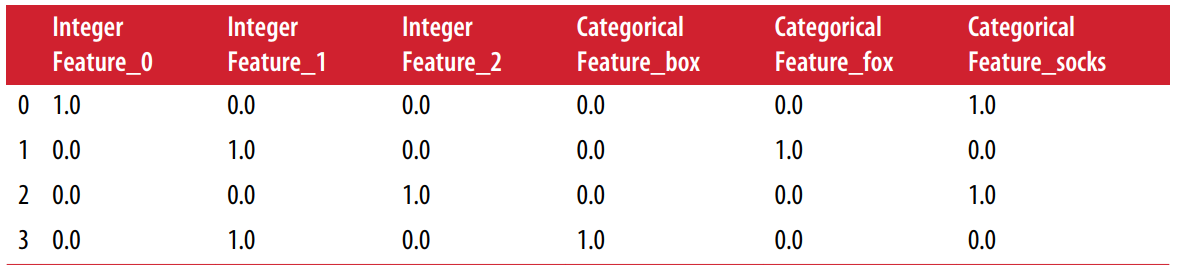
\includegraphics[scale=0.55]{Imagen_Machine/Tabla71}
		\end{tabular}
\end{table}
	
%   One-hot  instantánea 

\section{Binning, discretización, modelos lineales y árboles}
	
%	Binning, Discretization, Linear Models, and Trees

La mejor manera de representar los datos depende no sólo de la semántica de los datos, sino también del tipo de modelo que se va a utilizar.   Los modelos lineales y los  basados en árboles (como  árboles de decisión,  árboles potenciados por gradientes y  bosques aleatorios) son  dos grandes familias  muy comunes, tienen propiedades muy diferentes en cuanto a cómo funcionan con diferentes representaciones de características.  
 
Volvamos al conjunto de datos de regresión de Ondas que usamos en el capítulo \ref{Cap2}, esta  solo tiene una característica de entrada. Aquí  presentamos una comparación de un modelo de regresión lineal con  un árbol de  regresión sobre  este conjunto de datos (ver Figura \ref{Comparando01}):

	
\begin{lstlisting}%[frame=single]

In[11]:

   from sklearn.linear_model import LinearRegression
   from sklearn.tree import DecisionTreeRegressor
   
   X, y = mglearn.datasets.make_wave(n_samples=100)
   line = np.linspace(-3, 3, 1000, endpoint=False).reshape(-1, 1)
   
   reg = DecisionTreeRegressor(min_samples_split=3).fit(X, y)
   plt.plot(line, reg.predict(line), label="decision tree")
   
   reg = LinearRegression().fit(X, y)
   plt.plot(line, reg.predict(line), label="linear regression")
   plt.plot(X[:, 0], y, 'o', c='k')
   plt.ylabel("Regression output")
   plt.xlabel("Input feature")
   plt.legend(loc="best")
 
\end{lstlisting}

Como ya sabemos, los modelos lineales sólo pueden modelar relaciones lineales, que son líneas rectas en el caso de una sola característica. El árbol de decisión puede construir un modelo mucho más complejo sobre los datos. Sin embargo, esto depende fuertemente de la representación de los datos. Una manera de hacer que los modelos lineales sean más potentes en datos continuos es aplicar  {\ttfamily binning}\index{binning} (también conocido como discretización\index{discretización}) sobre la característica, para dividirla en múltiples características, como se describe a continuación.\\

\begin{figure}[h!]
	\centering
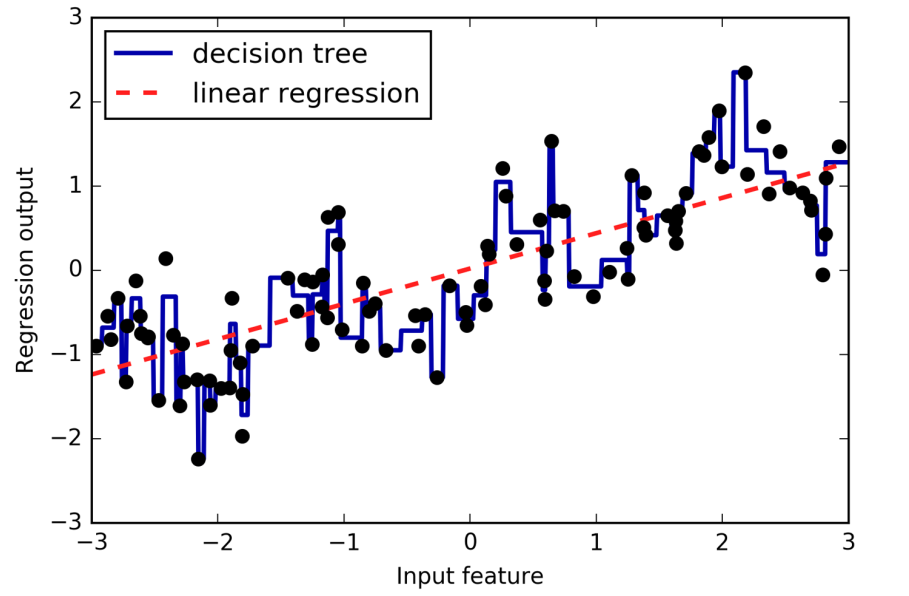
\includegraphics[scale=0.55]{Imagen_Machine/Comparando01}
	\caption{Comparación de regresión lineal y un árbol de decisión en el conjunto de datos de Onda}
	\label{Comparando01}
\end{figure}

Imaginamos una partición del rango de entrada para la característica (en este caso, los números
de –3 a 3) en un número fijo de intervalos (bins), por ejemplo 10. Un punto de datos será  representado por el intervalo que lo contenga. Para determinar esto, primero tenemos que definir los intervalos. En  este caso, definiremos 10 intervalos igualmente espaciados entre –3 y 3; utilizando la función 
{\ttfamily np.linspace}, gererando 11 entradas, que crearán 10 intervalos, que son
los espacios entre dos límites consecutivos:

\begin{lstlisting} 

In[12]:

   bins = np.linspace(-3, 3, 11)
   print("bins: {}".format(bins))

Out[12]:

    bins: [-3.  -2.4  -1.8  -1.2  -0.6  0.  0.6  1.2  1.8  2.4  3. ]

\end{lstlisting}


Aquí, el primer intervalo contiene todos los puntos de la  data con valores de características de
  \:  –3 \:    a  \:  –2.4, el segundo intervalo contiene todos los puntos con valores de características de \: –2,4 \: a \: -1.18,  y  así sucesivamente.


A continuación, registramos  cada punto de la  data en el intervalo que cae. Esto se puede calcular fácilmente usando la función {\ttfamily np.digitize}: \\


\begin{lstlisting}%[frame=single]

In[13]:

   which_bin = np.digitize(X, bins=bins)
   print("\nData points:\n", X[:5])
   print("\nBin membership for data points:\n", which_bin[:5])

Out[13]:

    Data points:
    [[-0.753]
     [ 2.704]
     [ 1.392]
     [ 0.592]
     [-2.064]]

   Bin membership for data points:
    [[ 4]
     [10]
     [ 8]
     [ 6]
     [ 2]]

\end{lstlisting}

	
Lo que hicimos aquí es transformar la característica de entrada continua única en el conjunto de datos de onda en una característica categórica que codifica en qué intervalo se encuentra un punto de datos. 

Para usar un modelo {\ttfamily scikit-learn }  sobre estos datos, transformamos esta característica discreta en una codificación one-hot,	usando el {\ttfamily OneHotEncoder} del módulo de pre-procesamiento. El {\ttfamily OneHotEncoder}  hace 	la misma codificación que {\ttfamily pandas.get\_dummies}, aunque realmente sólo actúa  sobre  variables categóricas que son enteros:\\

\begin{lstlisting}%[frame=single]

In[14]:

   from sklearn.preprocessing import OneHotEncoder
   # transform using the OneHotEncoder
   encoder = OneHotEncoder(sparse=False)
   # encoder.fit finds the unique values that appear in which_bin
   encoder.fit(which_bin)
   # transform creates the one-hot encoding
   X_binned = encoder.transform(which_bin)
   print(X_binned[:5])

Out[14]:

    [[ 0. 0. 0. 1. 0. 0. 0. 0. 0. 0.]
     [ 0. 0. 0. 0. 0. 0. 0. 0. 0. 1.]
     [ 0. 0. 0. 0. 0. 0. 0. 1. 0. 0.]
     [ 0. 0. 0. 0. 0. 1. 0. 0. 0. 0.]
     [ 0. 1. 0. 0. 0. 0. 0. 0. 0. 0.]]



\end{lstlisting}

Debido a que especificamos 10 intervalos, la data transformada {\ttfamily X\_binned} ahora se compone de 10 características:



\begin{lstlisting}%[frame=single]

In[15]:
   
   print("X_binned.shape: {}".format(X_binned.shape))

Out[15]:

    X_binned.shape: (100, 10)

\end{lstlisting}

Ahora construimos un nuevo modelo de regresión lineal y un nuevo modelo de árbol de decisión sobre la data   codificados  one-hot.   El resultado se visualiza en la Figura \ref{Comparando02}, junto con los límites  del intervalo, mostrados como líneas punteadas en negro:\\ 

\begin{lstlisting}%[frame=single]

In[16]:

   line_binned = encoder.transform(np.digitize(line, bins=bins))
   
   reg = LinearRegression().fit(X_binned, y)
   plt.plot(line, reg.predict(line_binned), label='linear regression binned')
   
   reg = DecisionTreeRegressor(min_samples_split=3).fit(X_binned, y)
   plt.plot(line, reg.predict(line_binned), label='decision tree binned')
   plt.plot(X[:, 0], y, 'o', c='k')
   plt.vlines(bins, -3, 3, linewidth=1, alpha=.2)
   plt.legend(loc="best")
   plt.ylabel("Regression output")
   plt.xlabel("Input feature")
   
\end{lstlisting}


\begin{figure}[h!]
	\centering
	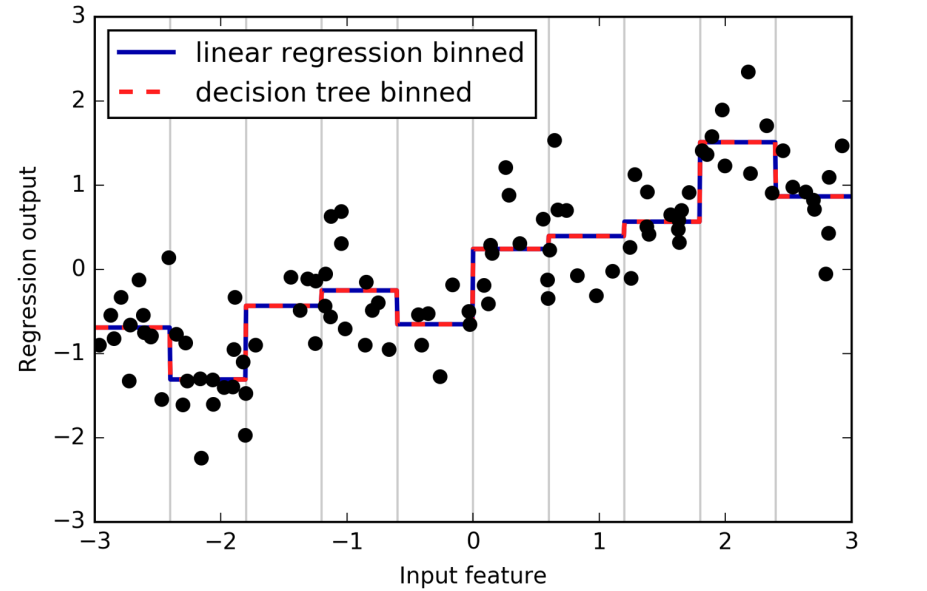
\includegraphics[scale=0.55]{Imagen_Machine/Comparando02}
	\caption{Comparación de la regresión lineal y la regresión de árbol de decisión sobre  las características en bins (agrupadas)}
	\label{Comparando02}
\end{figure}


La línea discontinua y la línea sólida están exactamente una encima de la otra, lo que significa que el modelo de regresión lineal y el árbol de decisiones hacen exactamente las mismas predicciones. Para cada intervalo, predicen un valor constante. Como las características son constantes dentro de cada intervalo, cualquier modelo debe predecir el mismo valor para todos los puntos dentro de un intervalo.

Comparando lo que los modelos aprendieron antes de combinar las características y después,
 vemos que el modelo lineal se volvió mucho más flexible, porque ahora tiene un valor diferente para cada intervalo, mientras que el modelo de árbol de decisión se volvió mucho menos flexible.
Las características  Binning generalmente no tienen ningún efecto beneficioso para los modelos basados en árboles, ya que estos modelos pueden aprender a dividir los datos en cualquier lugar. En cierto sentido, eso significa que los árboles de decisión pueden aprender lo que es más útil para predecir esta data.
 
Además, los árboles de decisión miran múltiples características a la vez, mientras que el binning generalmente se hace por cada característica. Sin embargo, el modelo lineal se benefició grandemente con la nueva transformación de los datos.\\

Si hay buenas razones para usar un modelo lineal en  un conjunto de datos en particular, por ejemplo, porque es muy grande y de alta dimensión, pero algunas características tienen relaciones no lineales, con la salida-binning puede ser una  manera de aumentar la potencia del modelo. 


\section{Interacciones y polinomios}

Otra manera de enriquecer una representación de características, particularmente para modelos lineales, es añadir  interacción de características  y  polinómicas de características a  los datos originales. Este tipo de ingeniería de características es frecuentemente usado  en el modelado estadístico, pero también es común en muchas aplicaciones prácticas de aprendizaje automático.\\

Como primer ejemplo, observe nuevamente la Figura \ref{Comparando02}. El modelo lineal aprendió un valor constante para cada intervalo en la dataset wave. Sin embargo, sabemos que los modelos lineales pueden aprender no solo las compensaciones, sino también las pendientes.
 Una forma de añadir una pendiente al modelo lineal sobre la data binned es  agregar la característica original (el eje x en la gráfica) nuevamente. Esto lleva a una dataset de  11 dimensiones, como se ve en la Figura \ref{Binned}:	
	

\begin{lstlisting}%[frame=single]

In[17]:

   X_combined = np.hstack([X, X_binned])
   print(X_combined.shape)

Out[17]:

    (100, 11)

In[18]:

   reg = LinearRegression().fit(X_combined, y)
   
   line_combined = np.hstack([line, line_binned])
   plt.plot(line, reg.predict(line_combined), 
            label='linear regression combined')
   
   for bin in bins:
       plt.plot([bin, bin], [-3, 3], ':', c='k')
       plt.legend(loc="best")
       
   plt.ylabel("Regression output")
   plt.xlabel("Input feature")
   plt.plot(X[:, 0], y, 'o', c='k')
   
\end{lstlisting}
	


\begin{figure}[h!]
	\centering
%	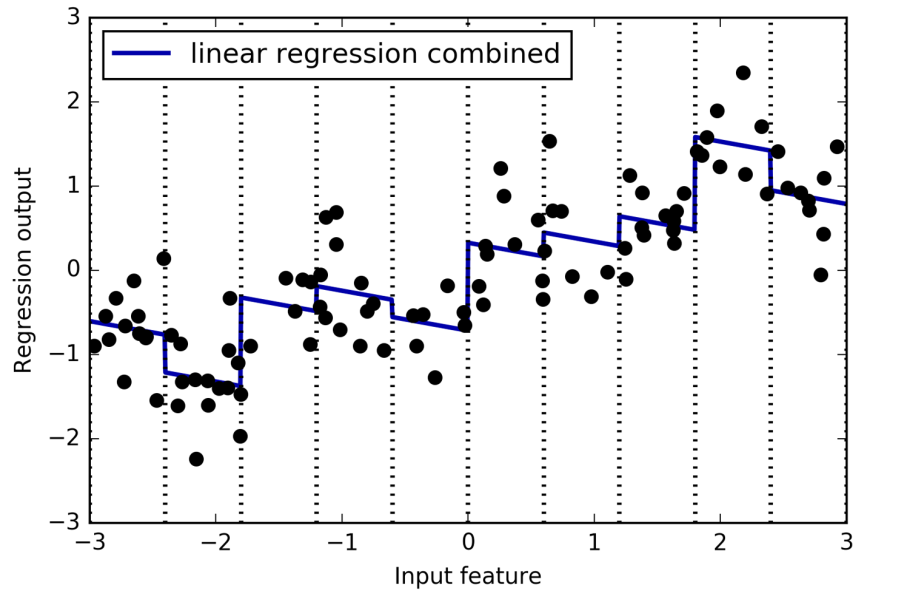
\includegraphics[scale=0.55]{Imagen_Machine/Binned}
    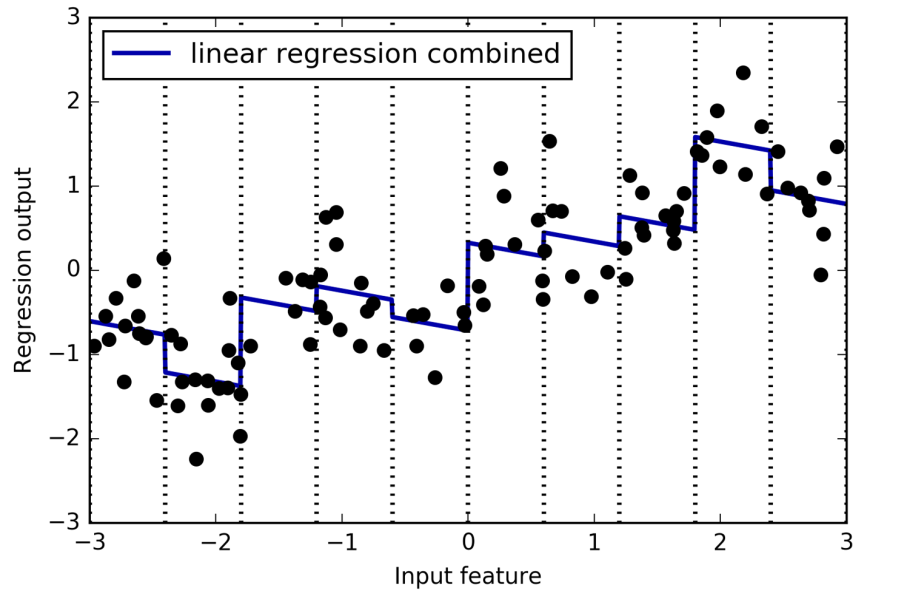
\includegraphics[scale=0.55]{Imagen_Machine/Binned}
	\caption{Regresión lineal usando características combinadas y una sola pendiente global}
	\label{Binned}
\end{figure}

En este ejemplo, el modelo aprendió una compensación  para cada intervalo, junto con una pendiente. La pendiente aprendida va hacia abajo, y se comparte a través de todos los intervalos; hay una sola característica del eje $x$, que tiene una sola pendiente. 

Debido a que la pendiente se comparte a través de todos los intervalos, no parece ser muy útil. Preferiríamos tener una pendiente separada para cada intervalo!   Podemos lograr esto añadiendo una caraterística  de interacción o producto que indica en qué intervalo se encuentra un punto de datos y dónde se encuentra en el eje x. Esta característica es un producto del intervalo indicador y de la característica original.  Vamos a crear este conjunto de datos:\\


\begin{lstlisting}%[frame=single]

In[19]:

   X_product = np.hstack([X_binned, X * X_binned])
   print(X_product.shape)

Out[19]:

    (100, 20)

\end{lstlisting}

 
La data ahora tiene 20 características: los  intervalos indicadores  en que un punto de la data está en él, y un producto de la característica original y el intervalo  indicador. Se puede pensar en el producto de la característica  como una copia separada de la característica del eje x para cada intervalo. Es la característica original dentro del intervalo, y cero en otro caso. La Figura  \ref{SeparaBin}  muestra el resultado del modelo lineal en esta nueva representación:

\begin{lstlisting}
	
In[20]:

   reg = LinearRegression().fit(X_product, y)
   
   line_product = np.hstack([line_binned, line * line_binned])
   plt.plot(line, reg.predict(line_product), 
            label='linear regression product')
   
   for bin in bins:
       plt.plot([bin, bin], [-3, 3], ':', c='k')
       
   plt.plot(X[:, 0], y, 'o', c='k')
   plt.ylabel("Regression output")
   plt.xlabel("Input feature")
   plt.legend(loc="best")


\end{lstlisting}


\begin{figure}[h!]
	\centering
	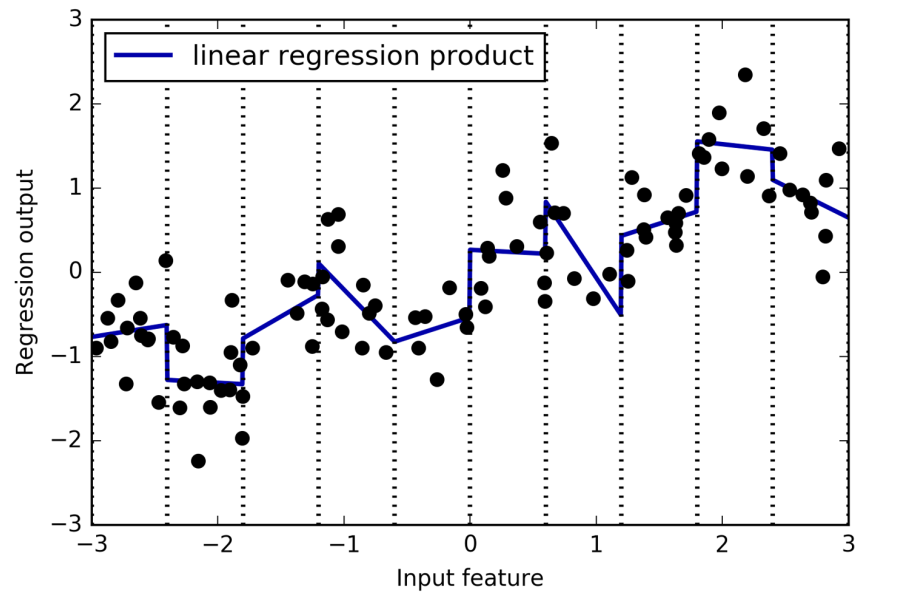
\includegraphics[scale=0.55]{Imagen_Machine/SeparaBin}
	\caption{Regresión lineal con una pendiente separada por intervalo}
	\label{SeparaBin}
\end{figure}

Como puedes ver, ahora cada intervalo  tiene su propia compensación y pendiente en este modelo.

Usar binning es una forma de expandir una característica continua. Otra es utilizar polinomios de las características originales. Para una característica dada $x$, podríamos considerar $ x**2, \: x**3, \: x**4, $ \: y así sucesivamente. Esto se implementa en {\ttfamily PolynomialFeatures} del módulo de preprocesamiento:

\begin{lstlisting}	
In[21]:

   from sklearn.preprocessing import PolynomialFeatures
   # include polynomials up to x ** 10:
   # the default "include_bias=True" adds a feature that's constantly 1
   poly = PolynomialFeatures(degree=10, include_bias=False)
   poly.fit(X)
   X_poly = poly.transform(X)
   
   
\end{lstlisting} 

El uso de  grado igual a  10, produce 10 características:

\begin{lstlisting}

In[22]:

   print("X_poly.shape: {}".format(X_poly.shape))

Out[22]:

    X_poly.shape: (100, 10)  
  
  \end{lstlisting}    
 
 Comparemos las entradas de {\ttfamily X\_poly} con las de X:\\
 
 \begin{lstlisting}%[frame=single]
 
In[23]:

   print("Entries of X:\n{}".format(X[:5]))
   print("Entries of X_poly:\n{}".format(X_poly[:5]))

Out[23]:
   
    Entries of X:
    [[-0.753]
     [ 2.704]
     [ 1.392]
     [ 0.592]
     [-2.064]]
    Entries of X_poly:
    [[    -0.753     0.567    -0.427      0.321  -0.242    0.182
          -0.137     0.103    -0.078      0.058]
    [      2.704     7.313    19.777     53.482  144.632  391.125
        1057.714  2860.360  7735.232  20918.278]
    [      1.392     1.938     2.697      3.754    5.226    7.274
          10.125    14.094    19.618     27.307]
    [      0.592     0.350     0.207      0.123    0.073    0.043
           0.025     0.015     0.009      0.005]
    [     -2.064     4.260    -8.791     18.144  -37.448   77.289
        -159.516   329.222  -679.478   1402.367]]

	



\end{lstlisting}



	Puede obtener la semántica de las características llamando al método {\ttfamily get\_feature\_names}, que proporciona el exponente para cada característica:
	
\begin{lstlisting}	
		
In[24]:

   print("Polynomial feature names:\n{}".format(poly.get_feature_names()))
   
Out[24]:
	
   Polynomial feature names:
   ['x0', 'x0^2', 'x0^3', 'x0^4', 'x0^5', 'x0^6', 'x0^7', 'x0^8', 'x0^9',
    'x0^10']
	
\end{lstlisting}
	

	
Puedes ver que la primera columna de {\ttfamily X\_poly} corresponde exactamente a X, mientras que las otras columnas son las potencias de la primera entrada. Es interesante ver lo grandes que pueden llegar a ser algunos de los valores. La segunda columna tiene entradas por encima de 20.000, órdenes de magnitud diferentes del resto. El uso de características polinómicas junto con un modelo de regresión lineal produce el modelo clásico de regresión polinómica (ver Figura \ref{Polinomio}):	

\begin{lstlisting}

In[25]:  # repetido erroe 26

   reg = LinearRegression().fit(X_poly, y)
   
   line_poly = poly.transform(line)
   plt.plot(line, reg.predict(line_poly), label='polynomial linear
            regression')
   plt.plot(X[:, 0], y, 'o', c='k')
   plt.ylabel("Regression output")
   plt.xlabel("Input feature")
   plt.legend(loc="best")

\end{lstlisting}



\begin{figure}[h!]
	\centering
	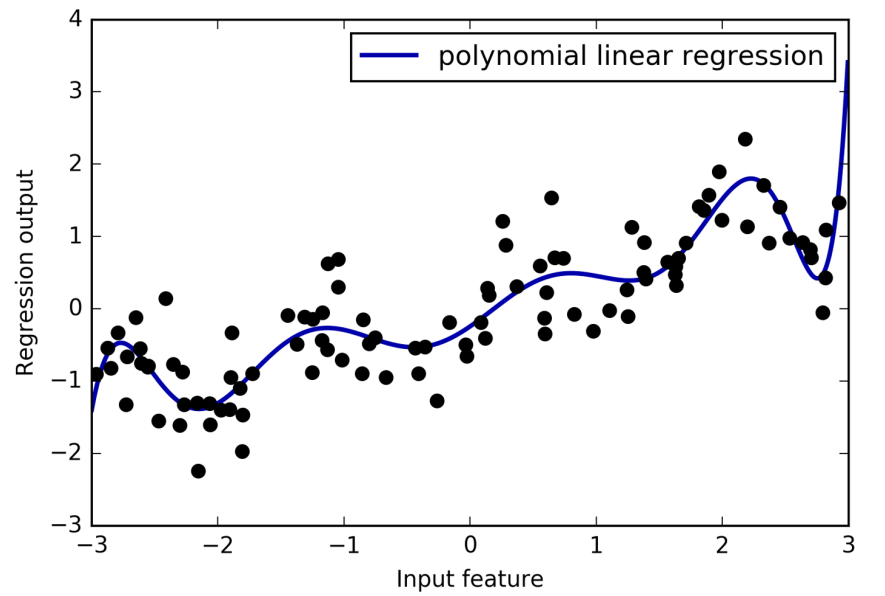
\includegraphics[scale=0.55]{Imagen_Machine/Polinomio}
	\caption{Regresión lineal con una pendiente separada por intervalo}
	\label{Polinomio}
\end{figure}


Como puedes ver, las características polinómicas producen un ajuste muy suave en estos datos unidimensionales. Sin embargo, los polinomios de alto grado tienden a comportarse de manera extrema en los límites o en regiones con pocos datos. \\

Como una comparación, aqui se presenta  un  modelo kernel SVM  aprendido sobre los datos originales, sin ninguna transformación de la data (ver Figura \ref{KernelCarat}):
	

\begin{lstlisting}

In[26]:   # error   26 repetido

  from sklearn.svm import SVR
  
  for gamma in [1, 10]:
      svr = SVR(gamma=gamma).fit(X, y)
      plt.plot(line, svr.predict(line), label='SVR gamma={}'.format(gamma))
      
  plt.plot(X[:, 0], y, 'o', c='k')
  plt.ylabel("Regression output")
  plt.xlabel("Input feature")
  plt.legend(loc="best")

  \end{lstlisting}
	
%   KernelCarat

\begin{figure}[h!]
	\centering
	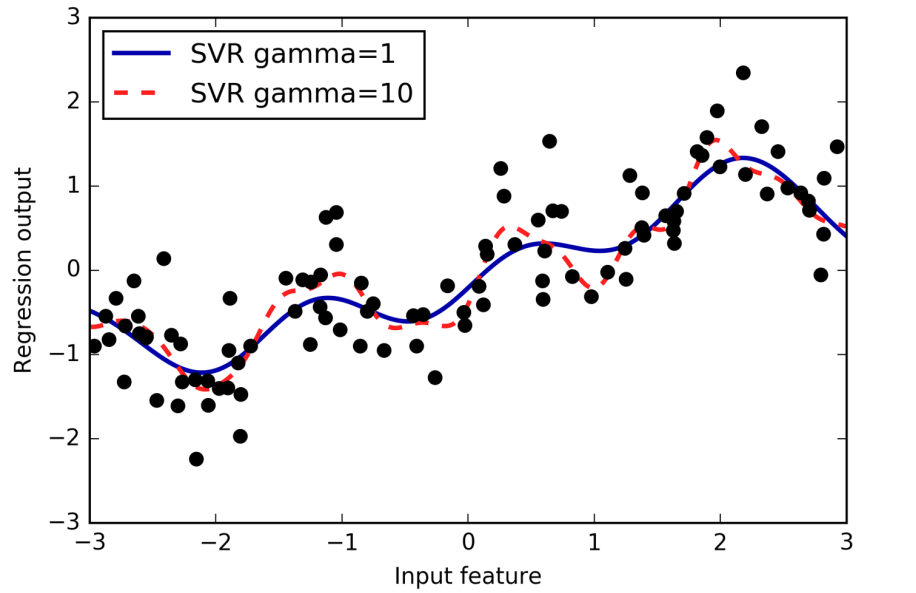
\includegraphics[scale=0.55]{Imagen_Machine/KernelCarat}
	\caption{Comparación de diferentes parámetros gamma para un SVM con el núcleo RBF}
	\label{KernelCarat}
\end{figure}


Usando un modelo más complejo, un SVM kernel, podemos aprender una predicción igualmente compleja de la regresión polinómica sin una transformación explícita de las características.


Como una aplicación más realista de interacciones y polinomios, veamos de nuevo el conjunto de datos de Boston Housing. Ya hemos utilizado características polinómicas sobre  este conjunto de datos en el capítulo \ref{Cap2}.  Ahora veamos cómo se construyeron estas características, y en qué medida las características polinómicas ayudan. Primero cargamos los datos y los reescalemos  entre 0 y 1 usando {\ttfamily MinMaxScaler}: \\	

 
\begin{lstlisting}%[frame=single]

In[27]:

   from sklearn.datasets import load_boston
   from sklearn.model_selection import train_test_split
   from sklearn.preprocessing import MinMaxScaler
   
   boston = load_boston()
   X_train, X_test, y_train, y_test = train_test_split(
        boston.data, boston.target, random_state=0)
       
   # rescale data
   scaler = MinMaxScaler()
   X_train_scaled = scaler.fit_transform(X_train)
   X_test_scaled = scaler.transform(X_test)

\end{lstlisting}


Ahora, extraemos características e interacciones polinómicas hasta el grado de 2:\\


\begin{lstlisting}%[frame=single]

In[28]:

   poly = PolynomialFeatures(degree=2).fit(X_train_scaled)
   X_train_poly = poly.transform(X_train_scaled)
   X_test_poly = poly.transform(X_test_scaled)
   print("X_train.shape: {}".format(X_train.shape))
   print("X_train_poly.shape: {}".format(X_train_poly.shape))

Out[28]:

   X_train.shape: (379, 13)
   X_train_poly.shape: (379, 105)


\end{lstlisting}%[frame=single]

 
Los datos originalmente tenían 13 características, que se ampliaron en 105 características  de interacción. Estas nuevas características representan todas las interacciones posibles entre dos características originales y por supuesto diferentes, así como el cuadrado de cada característica original. El grado 2 (degree = 2)   significa que miramos todas las características que son el producto de  dos características originales. La correspondencia exacta entre las características de entrada y salida se puede encontrar usando el método {\ttfamily get\_feature\_names}:\\

\begin{lstlisting}  %[frame=single]

In[29]:

   print("Polynomial feature names:\n{}".format(poly.get_feature_names()))

Out[29]:

   Polynomial feature names:
   ['1', 'x0', 'x1', 'x2', 'x3', 'x4', 'x5', 'x6', 'x7', 'x8', 'x9', 'x10',
   'x11', 'x12', 'x0^2', 'x0 x1', 'x0 x2', 'x0 x3', 'x0 x4', 'x0 x5', 
   'x0 x6','x0 x7', 'x0 x8', 'x0 x9', 'x0 x10', 'x0 x11', 'x0 x12', 'x1^2',
   'x1 x2','x1 x3', 'x1 x4', 'x1 x5', 'x1 x6', 'x1 x7', 'x1 x8', 'x1 x9', 
   'x1 x10','x1 x11', 'x1 x12', 'x2^2', 'x2 x3', 'x2 x4', 'x2 x5', 'x2 x6',
   'x2 x7', 'x2 x8', 'x2 x9', 'x2 x10', 'x2 x11', 'x2 x12', 'x3^2', 'x3 x4',
   'x3 x5', 'x3 x6', 'x3 x7', 'x3 x8', 'x3 x9', 'x3 x10', 'x3 x11', 'x3 x12', 
   'x4^2',  'x4 x5', 'x4 x6', 'x4 x7', 'x4 x8', 'x4 x9', 'x4 x10', 'x4 x11', 
   'x4 x12', 'x5^2', 'x5 x6', 'x5 x7', 'x5 x8', 'x5 x9', 'x5 x10', 'x5 x11', 
   'x5 x12', 'x6^2', 'x6 x7', 'x6 x8', 'x6 x9', 'x6 x10', 'x6 x11', 'x6 x12', 
   'x7^2', 'x7 x8', 'x7 x9', 'x7 x10', 'x7 x11', 'x7 x12', 'x8^2', 'x8 x9', 
   'x8 x10', 'x8 x11', 'x8 x12', 'x9^2', 'x9 x10', 'x9 x11', 'x9 x12',
    'x10^2', 'x10 x11', 'x10 x12', 'x11^2', 'x11 x12', 'x12^2']


\end{lstlisting}

La primera característica nueva es una característica constante, llamada "1".  Las siguientes 13 características son las características originales (llamadas "x0"{}  a "x12"). Luego sigue la primera característica al cuadrado ("x0\^{}2") y las combinaciones de la primera y con las demás características. \\

Comparemos el rendimiento usando Ridge en los datos con y sin interacciones:\\



\begin{lstlisting}%[frame=single]

In[30]:

   from sklearn.linear_model import Ridge
   ridge = Ridge().fit(X_train_scaled, y_train)
   print("Score without interactions: {:.3f}".format(
          ridge.score(X_test_scaled, y_test)))
   ridge = Ridge().fit(X_train_poly, y_train)
   print("Score with interactions: {:.3f}".format(
          ridge.score(X_test_poly, y_test)))

Out[30]:

    Score without interactions: 0.621
    Score with interactions: 0.753

\end{lstlisting}

Claramente, las interacciones y características polinómicas nos dieron un buen impulso en el rendimiento cuando se utiliza Ridge.  Aunque cuando se utiliza un modelo más complejo como un bosque aleatorio, la historia es un poco diferente, veamos en el siguiente ejemplo:


\begin{lstlisting}%[frame=single]


In[31]:

   from sklearn.ensemble import RandomForestRegressor
   rf = RandomForestRegressor(n_estimators=100).fit(X_train_scaled, y_train)
   print("Score without interactions: {:.3f}".format(
       rf.score(X_test_scaled, y_test)))
   rf = RandomForestRegressor(n_estimators=100).fit(X_train_poly, y_train)
   print("Score with interactions: {:.3f}".format(
           rf.score(X_test_poly, y_test)))

Out[31]:

    Score without interactions: 0.799
    Score with interactions: 0.763

\end{lstlisting}

Se puede ver que incluso sin características adicionales, el bosque aleatorio supera el rendimiento de Ridge. Añadiendo interacciones y polinomios disminuye ligeramente el rendimiento. 

\section{Transformaciones  univariables  no lineales}

Acabamos de ver que agregando características al cuadradas  o al cubo puede ayudar con 
los modelos lineales para  regresión. Hay otras transformaciones que a menudo resultan útiles para transformar ciertas características:  en particular, la aplicación de funciones matemáticas como $log,\: exp $  o $ \: sin$.  Mientras que en los modelos basados en árboles sólo  preocupa  el orden de las características, en los modelos lineales y las redes neuronales están muy ligadas a la escala y distribución de cada característica, y si existe es una relación no lineal entre la característica y el objetivo, se hace más difícil  modelar, particularmente en el caso de regresión. 
Las funciones  $log $  y  $ exp$  pueden ayudar ajustando las escalas relativas sobre los datos para que puedan ser capturados mejor por un modelo lineal o red neuronal. 
 
En el Capítulo \ref{Cap2} vimos una aplicación de esta técnica sobre los datos de precio de memoria RAM. Los
Las funciones $ sin $ y $ cos $ pueden ser útiles cuando se trata de datos que codifican patrones  periódicos.\\

La mayoría de los modelos funcionan mejor cuando cada característica (y en regresión también el objetivo) está distribuida vagamente gaussiana, es decir, un histograma de cada característica debe tener algo parecido a la familiar forma de "{}curva de campana". 
Usar transformaciones como $log$  y  $ exp$  es una forma simple y eficiente de lograr esto. Un caso particularmente común cuando tal transformación puede ser útil es cuando se trata de datos de recuento entero.  Por datos de recuento, nos referimos a características como "{}¿ Con qué frecuencia el usuario A inicia sesión ?"{}. Los recuentos nunca son negativos, y a menudo siguen patrones estadísticos particulares. Estamos utilizando una data sintética de conteos que tiene propiedades similares a las que se pueden encontrar en la naturaleza. Las características son todas de valor entero, mientras que la respuesta es continua:\\


\begin{lstlisting}%[frame=single]

In[32]:

   rnd = np.random.RandomState(0)
   X_org = rnd.normal(size=(1000, 3))
   
   w = rnd.normal(size=3)
   X = rnd.poisson(10 * np.exp(X_org))
   y = np.dot(X_org, w)

\end{lstlisting}


Veamos las primeras 10 entradas de la primera característica. Todos son valores enteros y positivos, pero aparte de eso es difícil distinguir un patrón particular. Si contamos la apariencia de cada valor, la distribución de valores se vuelve más clara:\\

\begin{lstlisting}%[frame=single]

In[33]:

   print("Number of feature appearances:\n{}".format(np.bincount(X[:, 0])))

Out[33]:
 
    Number of feature appearances:
    [28 38 68 48 61 59 45 56 37 40 35 34 36 26 23 26 27 21 23 23 18 21 10  9 
     17  9  7 14 12  7  3  8  4  5  5  3  4  2  4  1  1  3  2  5  3  8  2  5 
      2  1  2  3  3  2  2  3  3  0  1  2  1  0  0  3  1  0  0  0  1  3  0  1 
      0  2  0  1  1  0  0  0  0  1  0  0  2  2  0  1  1  0  0  0  0  1  1  0
      0  0  0  0  0  0  1  0  0  0  0  0  1  1  0  0  1  0  0  0  0  0  0  0
      1  0  0  0  0  1  0  0  0  0  0  0  0  0  0  0  0  0  0  0  1]
\end{lstlisting}

El valor 2 parece ser el más común, con 68 apariencias (el conteo siempre comienza en 0), y el conteo de valores más altos cae rápidamente. Sin embargo, hay algunos valores muy altos, como 134 apareciendo dos veces. Podemos visualizamos los conteos en la Figura \ref{HistoValores}:\\

\begin{lstlisting}%[frame=single]

In[34]:

   bins = np.bincount(X[:, 0])
   plt.bar(range(len(bins)), bins, color='w')
   plt.ylabel("Number of appearances")
   plt.xlabel("Value")

\end{lstlisting}


\begin{figure}[h!]
	\centering
	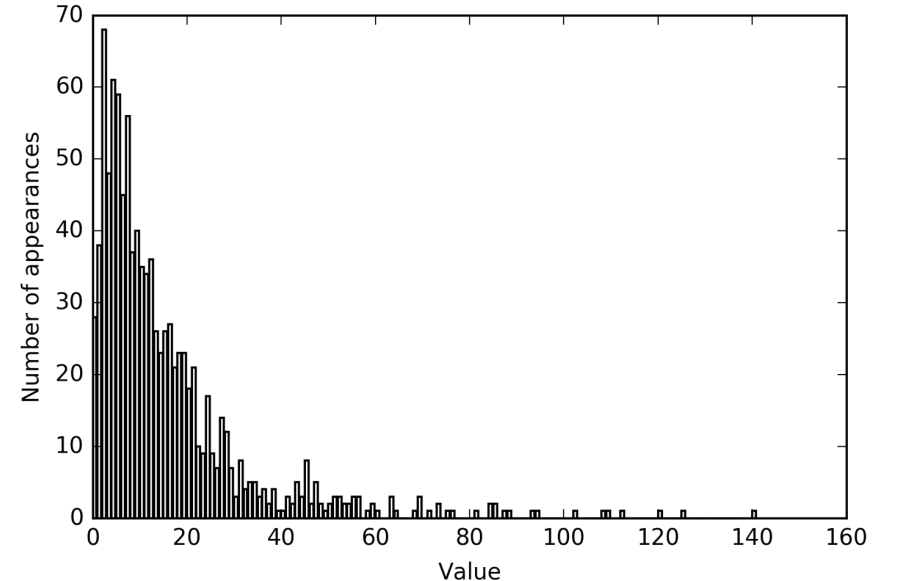
\includegraphics[scale=0.55]{Imagen_Machine/HistoValores}
	\caption{Histograma de los valores de las características de X[0]}
	\label{HistoValores}
\end{figure}

                       %                              \tiny
Las características  X[:, 1]  y  X[:, 2]  tienen propiedades similares. Este tipo de distribución de valores (muchos valores  muy pequeños y pocos muy grandes) es muy común en la práctica{\footnote{\scriptsize	{ Esta es una distribución de Poisson, que es bastante fundamental para contar datos}}}. Sin embargo, es algo que la mayoría de los modelos lineales no pueden manejar muy bien. Vamos a tratar de encajar una regresión  Ridge a este modelo:\\


\begin{lstlisting}%[frame=single]

In[35]:

   from sklearn.linear_model import Ridge
   X_train, X_test, y_train, y_test = train_test_split(X, y, random_state=0)
   score = Ridge().fit(X_train, y_train).score(X_test, y_test)
   print("Test score: {:.3f}".format(score))

Out[35]:

    Test score: 0.622

\end{lstlisting}


Como se puede ver  la puntuación $R^{2}$ relativamente baja, Ridge no fue capaz de capturar realmente la relación entre $X$ e $y$. Sin embargo, aplicando  una transformación logarítmica puede ayudar.  Debido a que el valor 0 aparece en la data (y el logaritmo no está definido en 0), no podemos aplicar $log$, pero tenemos que calcular $log(X + 1)$:\\


\begin{lstlisting}%[frame=single]

In[36]:

   X_train_log = np.log(X_train + 1)
   X_test_log = np.log(X_test + 1)
\end{lstlisting}


Después de la transformación, la distribución de los datos es menos asimétrica y  no tiene valores atípicos (outliers) tan  grandes (ver Figura \ref{HistoValores2}):\\
 
 
\begin{lstlisting}%[frame=single]

In[37]:

   plt.hist(np.log(X_train_log[:, 0] + 1), bins=25, color='gray')
   plt.ylabel("Number of appearances")
   plt.xlabel("Value")
\end{lstlisting}


\begin{figure}[h!]
	\centering
	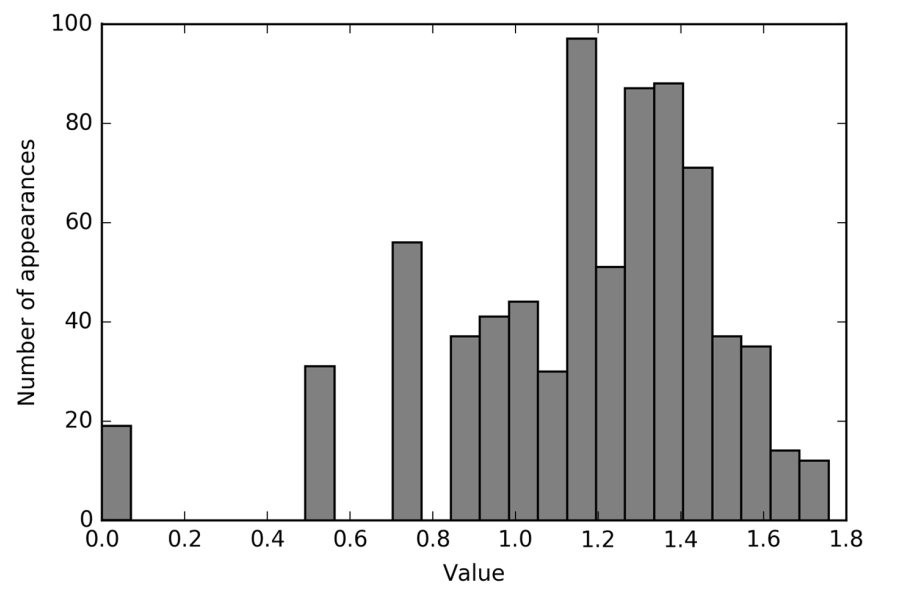
\includegraphics[scale=0.55]{Imagen_Machine/HistoValores2}
	\caption{Histograma de los valores de las características para X[0] después de la transformación logarítmica}
	\label{HistoValores2}
\end{figure}

La construcción de un modelo Ridge sobre  la data nueva  proporciona un ajuste mucho mejor:\\

\begin{lstlisting}%[frame=single]

In[38]:

   score = Ridge().fit(X_train_log, y_train).score(X_test_log, y_test)
   print("Test score: {:.3f}".format(score))

Out[38]:
   
    Test score: 0.875
\end{lstlisting}



Encontrar la transformación que funciona mejor para cada combinación de dataset y modelo es  un arte. En este ejemplo, todas las características tenían las mismas propiedades.  En la práctica esto se presenta raramente, y por lo general sólo un subconjunto de las características debe ser transformado, o a veces cada característica tiene que ser transformado de una manera diferente.   Como mencionamos anteriormente, este tipo de transformaciones son irrelevantes para los modelos basados en árboles, pero podrían ser esenciales para los modelos lineales.  A veces también es una buena idea transformar la variable objetivo $y$ en regresión. Tratar de predecir los conteos (por ejemplo, el número de órdenes) es una tarea muy común, y usar la transformación $ log(y + 1)$ a menudo ayuda{\footnote{\scriptsize Esta es una aproximación muy cruda del uso de la regresión de Poisson, que sería la solución adecuada desde un punto de vista probabilístico}}.\\

Como vieron en los ejemplos anteriores, el binning, los polinomios y las interacciones pueden tener una gran influencia en cómo funcionan los modelos en un conjunto de datos dado. 
 Esto es particularmente cierto para los modelos menos complejos como los modelos lineales y los modelos   naives Bayes. Por otra parte, los modelos basados en árboles,  a menudo son capaces de descubrir interacciones importantes, y no requieren la transformación explícitamente de los datos en la mayor parte de las veces.   Otros modelos, como   SVMs,  vecinos más cercanos  y  redes neuronales, a veces podrían beneficiarse del uso de binning, interacciones o polinomios, pero las implicaciones allí son generalmente mucho menos claras que en el caso de los modelos lineales.


\section{Selección automática de características}

Con tantas formas de crear nuevas características, puede sentirse tentado a aumentar la dimensionalidad de los datos más allá del número de características originales.  Sin embargo, agregar más características  hace que todos los modelos sean más complejos,  y  por lo tanto, aumenta la posibilidad de sobreajuste. Al agregar nuevas características o en caso de datas con alta dimensión,   puede ser una buena idea reducir la cantidad de características  solo a las más útiles, y descartar el resto. Esto puede conducir a modelos más simples que generalizan mejor. Pero  ¿ cómo se puede saber qué tan importante es una  característica?   Hay tres estrategias básicas: las estadísticas  univariante, la selección basada en modelos y la selección iterativa. Discutiremos los tres en detalle. Todos estos son métodos  supervisados, lo que significa que necesitan un objetivo para ajustar el modelo. Esto significa que necesitamos dividir los datos en entrenamiento y prueba, y   ajustar  la selección de características sólo en la parte de la  data de  entrenamiento.

\subsubsection{Estadísticas univariada}

En las estadísticas univariantes  calculamos si existe una relación estadísticamente significativa  entre cada característica y el objetivo. Luego, se seleccionan las características que se relacionan con la mayor confianza. En el caso de la clasificación,  esto también se conoce como
Análisis de Varianza (ANOVA). Una propiedad clave de estas pruebas es que son univariadas, lo que significa que sólo se considera cada característica en foma individual.  En consecuencia, una característica se descartará si sólo es informativo cuando se combina con otra característica.  Las pruebas univariadas suelen ser muy rápidas de calcular y no requieren la construcción de un modelo. Por otro lado, son completamente independientes del modelo que se desea aplicar después de la selección de características.\\

Para usar la selección de características univariadas en {\ttfamily scikit-learn}, debe elegir una prueba,  \:  generalmente  para clasificación  \:  {\ttfamily f\_classif} \: (por defecto)  y  para regresión  {\ttfamily f\_regression}, y un método para descartar características basadas en los $p$-valoes  determinados en la prueba.  Todos los métodos para descartar parámetros usan un umbral para descartar todas las características con  un $p$-valor alto (lo que significa que es poco probable que estén relacionados con el objetivo). Los métodos  difieren en cómo calculan este umbral, siendo los más simples {\ttfamily SelectKBest}, que selecciona un número fijo  de $k$  características, y el {\ttfamily SelectPercentile}, que selecciona  un porcentaje fijo de características. Apliquemos la selección de características para clasificación sobre la  cancer dataset. Para hacer la tarea un poco más difícil, añadiremos algunas características de ruido no informativa a los datos. Esperamos que la selección de características sea capaz de identificar las características que no son informativas y eliminarlas:


\begin{lstlisting}%[frame=single]

In[39]:

   from sklearn.datasets import load_breast_cancer
   from sklearn.feature_selection import SelectPercentile
   from sklearn.model_selection import train_test_split
   
   cancer = load_breast_cancer()
   
   # get deterministic random numbers
   rng = np.random.RandomState(42)
   noise = rng.normal(size=(len(cancer.data), 50))
   # add noise features to the data
   # the first 30 features are from the dataset, the next 50 are noise
   X_w_noise = np.hstack([cancer.data, noise])
   
   X_train, X_test, y_train, y_test = train_test_split(
       X_w_noise, cancer.target, random_state=0, test_size=.5)
   # use f_classif (the default) and SelectPercentile to select 
   # 50% of features 
   select = SelectPercentile(percentile=50)
   select.fit(X_train, y_train)
   # transform training set
   X_train_selected = select.transform(X_train)

   print("X_train.shape: {}".format(X_train.shape))
   print("X_train_selected.shape: {}".format(X_train_selected.shape))

Out[39]:

    X_train.shape: (284, 80)
    X_train_selected.shape: (284, 40)

\end{lstlisting}


Como se puede ver, el número de características se redujo de  80  a  40 (50 por ciento del número original de características). Podemos averiguar qué características se han seleccionado utilizando el método {\ttfamily get\_support}, que devuelve una máscara booleana de las características seleccionadas (visualizada en la Figura \ref{SelecioPercet}):




\begin{lstlisting}%[frame=single]

In[40]:

   mask = select.get_support()
   print(mask)
   # visualize the mask -- black is True, white is False
   plt.matshow(mask.reshape(1, -1), cmap='gray_r')
   plt.xlabel("Sample index")

Out[40]:

    [ True True True True True True True True True False True False
      True True True True True True False False True True True True
      True True True True True True False False False True False True
      False False True False False False False True False False True False
      False True False True False False False False False False True False
      True False False False False True False True False False False False
      True True False True False False False False]


\end{lstlisting}




\begin{figure}[h!]
	\centering
	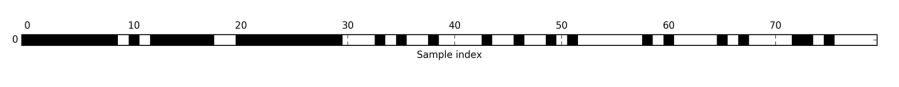
\includegraphics[scale=0.55]{Imagen_Machine/SelecioPercet}
	\caption{Características seleccionadas por SelectPercentile}
	\label{SelecioPercet}
\end{figure}



Como se puede ver en la visualización de la máscara, la mayoría de las características seleccionadas son las características originales, y la mayoría de las características de ruido se eliminaron. Sin embargo, 
la recuperación de las características originales no es perfecta. Vamos a comparar el rendimiento de la regresión logística en todas las características contra el rendimiento utilizando sólo las características seleccionadas:


\begin{lstlisting}%[frame=single]

In[41]:

   from sklearn.linear_model import LogisticRegression
   
   # transform test data
   X_test_selected = select.transform(X_test)
   
   lr = LogisticRegression()
   lr.fit(X_train, y_train)
   print("Score with all features: {:.3f}".format(lr.score(X_test, y_test)))
   lr.fit(X_train_selected, y_train)
   print("Score with only selected features: {:.3f}".format(
       lr.score(X_test_selected, y_test)))

Out[41]:

    Score with all features: 0.930
    
\end{lstlisting}

En este caso, la eliminación de las características de ruido mejoró el rendimiento, aunque algunos
de las características originales se perdieron. Este fue un ejemplo sintético  simple, y los resultados en datos reales suelen ser mixtos.

La selección de características univariadas puede ser muy útil, sin embargo, si hay un gran número de características que crean un modelo,  entonces no es factible, o si se sospecha que muchas características  son completamente {\bf{no} } informativas.

\subsection{Selección de características basada en modelos}

 La selección de características basada en un  modelo usa un modelo de aprendizaje automático supervisado para juzgar la  importancia de cada característica, y conserva solo las más importantes. 
 El modelo supervisado  que se usa para la selección de características  no necesita ser el mismo modelo que se usa para el modelo supervisado final.   El modelo de selección de características debe proporcionar alguna medida de importancia para cada característica, para que puedan ser clasificadas.

 Los árboles de decisión y los modelos basados árbol de decisión proporcionan un atributo  {\ttfamily feature\_importances\_}, que codifica directamente la importancia de cada característica.   Los modelos lineales tienen coeficientes, que también  pueden ser usados  para capturar las importancias de características considerando los valores absolutos.   Como vimos en el capítulo \ref{Cap2}, los modelos lineales con penalización L1 el aprendizaje de los  coeficientes sparse, que sólo utilizan un pequeño subconjunto de características.   Esto se puede ver como una forma de selección de características para el propio modelo, pero también se puede utilizar como un paso de preprocesamiento para seleccionar características para otro modelo. 
 En contraste con la selección univariable, la selección basada en modelos considera todas las características a la vez, y así puede capturar interacciones (si el modelo puede capturarlas).
 
  Para usar la selección de características basada en modelos, necesitamos usar el transformador {\ttfamily SelectFromModel}:\\


\begin{lstlisting}%[frame=single]

In[42]:
 
   from sklearn.feature_selection import SelectFromModel
   from sklearn.ensemble import RandomForestClassifier
   select = SelectFromModel(
            RandomForestClassifier(n_estimators=100, random_state=42),
            threshold="median")
       
\end{lstlisting}

La clase {\ttfamily SelectFromModel} selecciona todas las características que tienen una medida de importancia de la característica (según lo dispuesto por el modelo supervisado) mayor que el umbral proporcionado.  Para obtener un resultado comparable a lo que obtuvimos con la selección de características univariadas, utilizamos la mediana como un umbral, de modo que se seleccionará la mitad de las características.  Utilizamos un clasificador de bosques aleatorio con 100 árboles para calcular la importancia de las características. Este es un modelo muy  complejo y mucho más potente que el uso de pruebas univariadas. 
 


Ahora ajustemos el modelo:\\


\begin{lstlisting}%[frame=single]

In[43]:

   select.fit(X_train, y_train)
   X_train_l1 = select.transform(X_train)
   print("X_train.shape: {}".format(X_train.shape))
   print("X_train_l1.shape: {}".format(X_train_l1.shape))

Out[43]:
   
   X_train.shape: (284, 80)
   X_train_l1.shape: (284, 40)
   
\end{lstlisting}


Una vez más, podemos ver las características que fueron seleccionados (Figura \ref{SelecioPercet2}):

\begin{lstlisting}

In[44]:

   mask = select.get_support()
   # visualize the mask -- black is True, white is False
   plt.matshow(mask.reshape(1, -1), cmap='gray_r')
   plt.xlabel("Sample index")
   
\end{lstlisting}


\begin{figure}[h!]
	\centering
	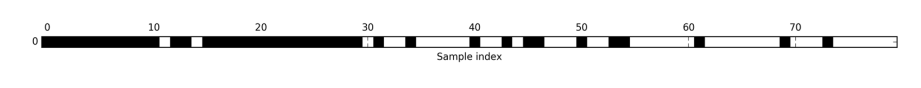
\includegraphics[scale=0.55]{Imagen_Machine/SelecioPercet2}
	\caption{Características seleccionadas por {\ttfamily SelectFromModel} usando el  {\ttfamily  RandomForestClassifier}}
	\label{SelecioPercet2}
\end{figure}


Esta vez, todas menos dos de las características originales fueron seleccionadas. Debido a que especificamos  40 características a seleccionar, algunas de las características de ruido también se seleccionaron. Veamos el rendimiento o desempeño:\\

\begin{lstlisting}%[frame=single]

In[45]:

   X_test_l1 = select.transform(X_test)
   score = LogisticRegression().fit(X_train_l1, y_train).score(X_test_l1,
                                                                y_test)
   print("Test score: {:.3f}".format(score))

Out[45]:
    
    Test score: 0.951

\end{lstlisting}

Con la mejor selección de característica, también hemos ganado algunas mejoras aquí.

\subsubsection{Selección iterativa de características}

En las pruebas univariates no usamos ningún modelo, mientras que en la selección basada en modelo
usamos un solo modelo  para seleccionar características. Ahora para la  selección iterativa de características, se construyen una serie de modelos, con un número variable de características. 

 Hay dos métodos básicos: comenzar sin características y agregando características una por una hasta que se alcance algún criterio de parada, o comenzando con todas las características y eliminar las características una por una hasta que se detenga por algún criterio de parada.   Debido a que se construyen una serie de modelos, estos métodos son mucho más  costoso computacionalmente  que los métodos que discutimos anteriormente. Un método  particular de este tipo es la eliminación recursiva de características (RFE, recursive feature elimination), que comienza 
 con todas las  características, crea un modelo y descarta la característica menos importante de acuerdo con el modelo.  Luego se construye un nuevo modelo utilizando todas las 
 características excepto las descartadas, y así sucesivamente hasta sólo queda un número pre-especificado de características. Para que esto funcione, el modelo usado para la selección debe proporcionar alguna forma de determinar la importancia de la característica, como fue el caso de la selección basada en el modelo. 

Aquí, usamos el mismo modelo de bosque aleatorio que empleamos anteriormente,  los resultados obtenidos
se muestran en la Figura \ref{SelecioPercet3}:


\begin{lstlisting}%[frame=single]

In[46]:

   from sklearn.feature_selection import RFE
   select = RFE(RandomForestClassifier(n_estimators=100, random_state=42),
                n_features_to_select=40)
                
   select.fit(X_train, y_train)
   # visualize the selected features:
   mask = select.get_support()
   plt.matshow(mask.reshape(1, -1), cmap='gray_r')
   plt.xlabel("Sample index")

\end{lstlisting}



\begin{figure}[h!]
	\centering
	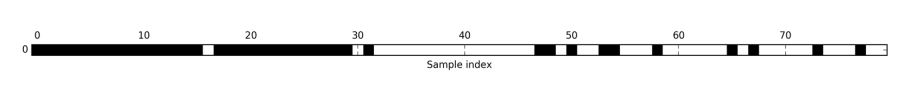
\includegraphics[scale=0.55]{Imagen_Machine/SelecioPercet3}
	\caption{Características seleccionadas por eliminación de características recursivas 
		con el modelo de clasificador bosques aleatorio}
	\label{SelecioPercet3}
\end{figure}

La selección de las características mejoró en comparación con la selección univariable y basada en modelos, pero una de las características todavía se perdió. Ejecutando  este código también toma mucho más tiempo que la selección basada en modelos, porque un modelo de bosque aleatorio se entrena 40 veces, una vez por cada característica que se elimina. 

Vamos a probar la precisión del modelo de regresión logística cuando se utiliza RFE para la selección de características:\\


\begin{lstlisting}%[frame=single]

In[47]:

   X_train_rfe= select.transform(X_train)
   X_test_rfe= select.transform(X_test)
   
   score = LogisticRegression().fit(X_train_rfe, y_train).score(X_test_rfe, y_test)
   print("Test score: {:.3f}".format(score))

Out[47]:

    Test score: 0.951

\end{lstlisting}


También podemos usar el modelo usado dentro del RFE para hacer predicciones. Esto usa sólo el conjunto de características que fue seleccionado:\\

\begin{lstlisting}%[frame=single]

In[48]:

   print("Test score: {:.3f}".format(select.score(X_test, y_test)))

Out[48]:

    Test score: 0.951


\end{lstlisting}


Aquí, el rendimiento del bosque aleatorio utilizado dentro del RFE es el mismo que se
logró entrenando un modelo de regresión logística sobre las características seleccionadas. En
en otras palabras, una vez que hemos seleccionado las características correctas, el modelo lineal funciona  también  como el bosque aleatorio.\\

 Si no está seguro qué características  seleccionar  como entrada para sus algoritmos de aprendizaje automático, la selección automática de características puede ser muy útil.  También es ideal para reducir la cantidad de características  necesarias, por ejemplo, para acelerar  la predicción o permitir modelos más interpretables. En la mayoría de los casos del mundo real,  la aplicación de selección de características es  poco probable que proporcione grandes ganancias en el rendimiento. Sin embargo, sigue siendo una herramienta valiosa en la caja de herramientas  del ingeniero de características.
   

\section{Utilizando conocimiento experto}


La ingeniería de características es a menudo un lugar importante para utilizar el conocimiento experto a una   aplicación particular. Si bien el propósito del aprendizaje automático en muchos casos es evitar
 crear un conjunto de reglas diseñadas por expertos, eso no significa que el conocimiento previo de
la aplicación o dominio debe descartarse.

Con frecuencia, los expertos en el área o experiencias  pueden ayudar en identificar características
útiles que son mucho más informativas que la representación inicial 
de la data.  Imagina que trabajas para una agencia de viajes y quieres predecir los precios de vuelo. 
Supongamos que tiene un registro de precios de diferentes  aerolíneas con fechas, lugar de salida
y destinos. Un modelo de aprendizaje automático podría ser capaz de construir un buen  modelo  a partir de estos datos.  Sin embargo, algunos factores importantes en los precios de los vuelos no se pueden aprender.
Por ejemplo, los vuelos suelen ser más caros durante los meses pico de vacaciones y
alrededor de los días festivos.
Si bien las fechas de algunos días festivos (como Navidad) son fijas, y
su efecto, por lo tanto, se puede aprender a partir de la fecha, otros pueden depender de las fases
de la luna (como los días de Hanukkah y Pascua) o ser establecido por las autoridades (como las vacaciones escolares). Estos eventos no  pueden  ser  aprendidos de la data si cada vuelo sólo se registra
usando la fecha (Gregoriana).  Sin embargo, es fácil agregar una característica  que codifique si un
el vuelo fue antes o después de un feriado público o escolar. 
De esta manera, el conocimiento previo sobre la naturaleza de la tarea se puede codificar en características para ayudar al algoritmo de aprendizaje automático.
 Agregar características no obliga a un algoritmo de aprendizaje automático a usarlo, e incluso si la información de vacaciones resulta no ser informativa  para los precios de los vuelos, aumentar los datos con esta información no hace daño. \\
 
 
Ahora veremos un caso particular de uso de conocimiento experto, aunque en este caso
podría llamarse más legítimamente "{}sentido común"{}.  La tarea es predecir el alquiler de bicicletas frente a la casa de Andreas.\\


En Nueva York, Citi Bike opera una red de estaciones de alquiler de bicicletas con un sistema de  suscripción.  Las estaciones están por toda la ciudad y proporcionan una manera conveniente de llegar
alrededor. Los datos de alquiler de bicicletas se hacen públicos de forma anónima y se han analizado de varias maneras.   La tarea que queremos resolver es predecir   cuántas personas alquilarán una bicicleta frente a la casa de Andreas en una hora y un día determinado, conociendo si hay alguna persona interesada  se le dejarán bicicletas.   Primero cargamos los datos de agosto de 2015 para esta estación en particular como una {\ttfamily Data Frame} de  {\ttfamily pandas}. Remuestreamos la data en intervalos de tres horas para obtener las principales tendencias por cada día:\\

\begin{lstlisting}%[frame=single]

In[49]:

   citibike = mglearn.datasets.load_citibike()


In[50]:

   print("Citi Bike data:\n{}".format(citibike.head()))

Out[50]:

    Citi Bike data:
    starttime
    2015-08-01 00:00:00 3.0
    2015-08-01 03:00:00 0.0
    2015-08-01 06:00:00 9.0
    2015-08-01 09:00:00 41.0
    2015-08-01 12:00:00 39.0
    Freq: 3H, Name: one, dtype: float64

\end{lstlisting}

El siguiente ejemplo muestra una visualización de las frecuencias de alquiler para todo el mes (Figura \ref{Bike1}):\\
   %     marca de tiempo de Unix 

\begin{lstlisting}%[frame=single]

In[51]:

   plt.figure(figsize=(10, 3))
   xticks = pd.date_range(start=citibike.index.min(), 
                           end=citibike.index.max(), freq='D')
   plt.xticks(xticks, xticks.strftime("%a %m-%d"), rotation=90, ha="left")
   plt.plot(citibike, linewidth=1)
   plt.xlabel("Date")
   plt.ylabel("Rentals")

\end{lstlisting}

\begin{figure}[h!]
	\centering
%	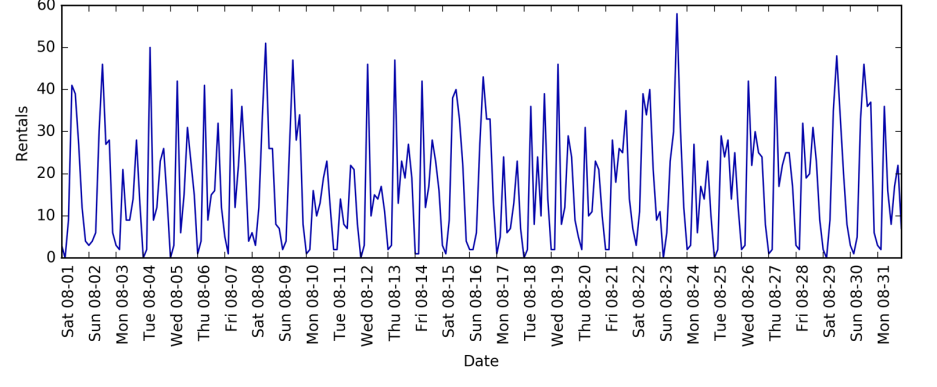
\includegraphics[scale=0.55]{Imagen_Machine/Bike1}
    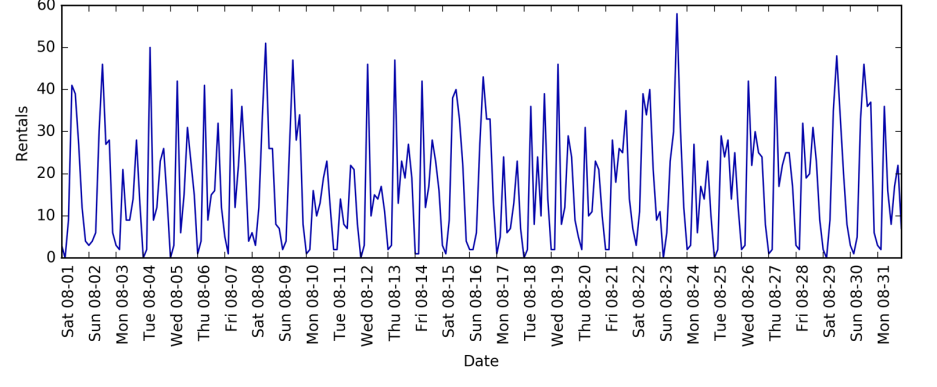
\includegraphics[scale=0.55]{Imagen_Machine/Bike1.png}
	\caption{Número de alquiler de bicicletas en el tiempo para una estación de Citi Bike seleccionada}
	\label{Bike1}
\end{figure}

Si observamos la data, podemos distinguir claramente día y noche para cada ínterval de 24 horas. Los patrones para los días de semana y los fines de semana también parecen ser muy diferentes.  Al evaluar una tarea de predicción en una serie temporal como esta, por lo general queremos aprender del pasado y predecir para el futuro.   Esto significa que al hacer una división en el conjunto de entrenamiento y de pruebas, queremos utilizar todos los datos hasta una fecha determinada como el conjunto de entrenamiento y todos los datos anteriores a esa fecha como el conjunto de pruebas.   
Así es como usualmente usamos la predicción de series de tiempo: dado todo lo que sabemos sobre alquileres en el pasado, ¿Qué crees que sucederá mañana? Utilizaremos los primeros 184 puntos de datos, correspondientes a los primeros 23 días, como el conjunto de entrenamiento, y los 64 puntos de datos restantes, correspondientes a los 8 días restantes, como el conjunto de pruebas.
 
La única característica que estamos utilizando en la tarea de predicción es la fecha y la hora en que se produjo un número particular de alquileres. Por lo tanto, la característica  de entrada es la fecha y hora, digamos, 2015-08-01 00:00:00- y la salida es el número de alquileres en las siguientes tres horas (tres en este caso, de acuerdo con  la {\ttfamily DataFrame}).

Una  manera común de que las fechas se almacenan en las computadoras está utilizando el tiempo POSIX, el cual  es el número de segundos desde enero de 1970 00:00:00 (también conocido como el comienzo del tiempo Unix). Como un primer intento, podemos utilizar esta única característica de entero único como la representación de la data:\\

\begin{lstlisting}%[frame=single]

In[52]:

   # extract the target values (number of rentals)
   y = citibike.values
   # convert the time to POSIX time using "%s"
   X = citibike.index.astype("int64").values.reshape(-1, 1) // 10**9
   # Genera error 
   # X = citibike.index.strftime("%s").astype("int").reshape(-1, 1)
   # por  version anterior
     
\end{lstlisting}

Primero definimos una función para dividir en el conjuntos de entrenamiento y prueba, construir el modelo,
y visualiza el resultado: 

\begin{lstlisting}

In[54]:

   # use the first 184 data points for training, and the rest for testing
   n_train = 184
   
   # function to evaluate and plot a regressor on a given feature set
   def eval_on_features(features, target, regressor):
       # split the given features into a training and a test set
       X_train, X_test = features[:n_train], features[n_train:]
       # also split the target array
       y_train, y_test = target[:n_train], target[n_train:]
       regressor.fit(X_train, y_train)
       print("Test-set R^2: {:.2f}".format(regressor.score(X_test, y_test)))
       y_pred = regressor.predict(X_test)
       y_pred_train = regressor.predict(X_train)
       plt.figure(figsize=(10, 3))
       
       plt.xticks(range(0, len(X), 8), xticks.strftime("%a %m-%d"), 
                  rotation=90, ha="left")
                  
       plt.plot(range(n_train), y_train, label="train")
       plt.plot(range(n_train, len(y_test) + n_train), y_test, '-',
                 label="test")
       plt.plot(range(n_train), y_pred_train, '--', 
                label="prediction train")
       
       plt.plot(range(n_train, len(y_test) + n_train), y_pred, '--',
                label="prediction test")
       plt.legend(loc=(1.01, 0))
       plt.xlabel("Date")
       plt.ylabel("Rentals")

\end{lstlisting}

Como vimos antes,  los bosques aleatorios requieren muy poco preprocesamiento en los datos, lo que hace que 
este parezca un buen modelo para empezar. Usamos la característica X de tiempo POSIX,  y pasamos  a un regresor de bosque aleatorio  la función {\ttfamily  eval\_on\_features}. La Figura \ref{POSIX} muestra el resultado:\\

\begin{lstlisting}%[frame=single]

In[55]:

   from sklearn.ensemble import RandomForestRegressor
   regressor = RandomForestRegressor(n_estimators=100, random_state=0)
   plt.figure()
   eval_on_features(X, y, regressor)

Out[55]:

    Test-set R^2: -0.04

\end{lstlisting}

\begin{figure}[h!]
	\centering
	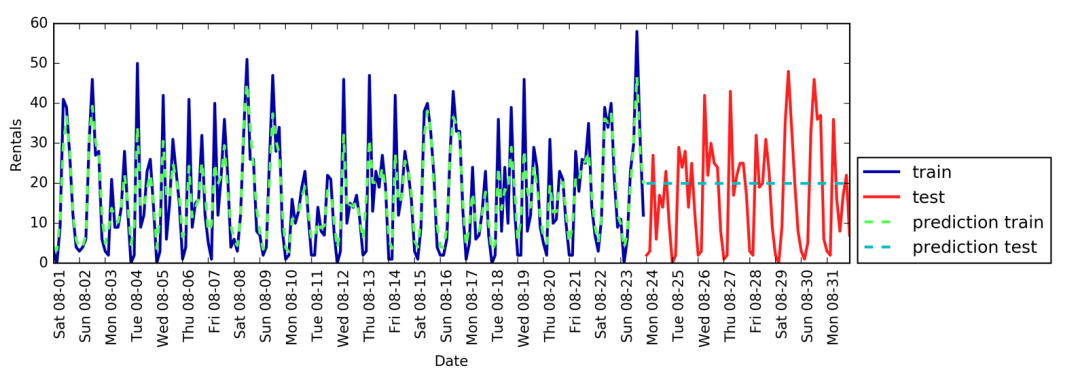
\includegraphics[scale=0.55]{Imagen_Machine/POSIX}
	\caption{Predicciones hechas por un bosque aleatorio usando sólo el tiempo POSIX}
	\label{POSIX}
\end{figure}

Las predicciones sobre el conjunto de entrenamiento son muy buenas, como es habitual para los bosques aleatorios; sin embargo, para el conjunto de pruebas, se predice una línea constante. El $R^{2}$ es -0.03, lo que significa que no aprendimos nada. ¿Qué pasó? \\

El problema radica en la combinación de la característica y el bosque aleatorio. 
El valor de la característica  de tiempo POSIX para el conjunto de prueba está fuera del rango de los valores de la característica en el conjunto de entrenamiento: los puntos en el conjunto de prueba tienen marcas de tiempo que son posteriores a todos los puntos en el conjunto de entrenamiento. 

Los árboles, y por lo tanto los bosques aleatorios, no pueden extrapolarse a rangos fuera del conjunto de entrenamiento. El resultado es que el modelo simplemente predice el valor objetivo del punto más cercano en el conjunto de entrenamiento, que es la última vez que observó cualquier dato.   Claramente podemos hacer algo mejor que esto. Aquí es donde entra nuestro "{}conocimiento experto". Al observar las cifras de alquiler en la data de entrenamiento, dos factores parecen ser muy importantes: la hora del día y el día de la semana.

 Por lo tanto, vamos a añadir estas dos características. Realmente no podemos aprender nada de la hora POSIX, por lo que sacamos esa característica. Primero, usemos sólo la hora del día. Como muestra la Figura \ref{DiaHora}, ahora las predicciones tienen el mismo patrón para cada día de la semana:

\begin{lstlisting}%[frame=single]

In[56]:

   X_hour = citibike.index.hour.values.reshape(-1, 1) 
   #  Error version  X_hour = citibike.index.hour.reshape(-1, 1)
   eval_on_features(X_hour, y, regressor)

Out[56]:

    Test-set R^2: 0.60
 
\end{lstlisting}


\begin{figure}[h!]
	\centering
	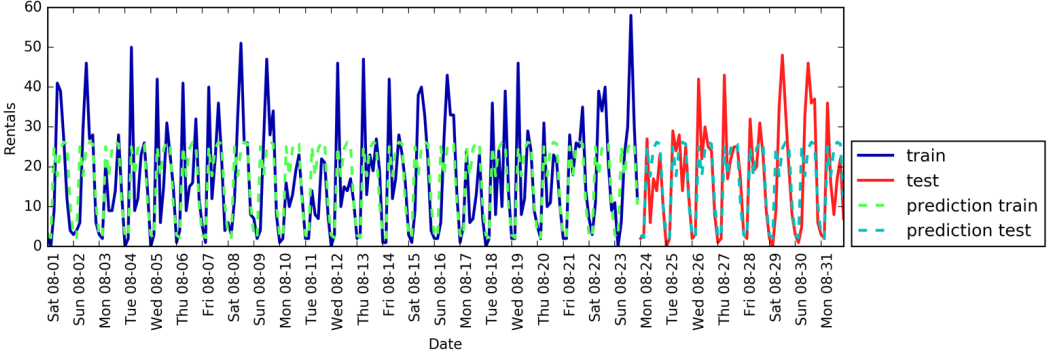
\includegraphics[scale=0.55]{Imagen_Machine/DiaHora}
	\caption{Predicciones hechas por un bosque al azar usando sólo la hora del día}
	\label{DiaHora}
\end{figure}


El $R^{2}$  mejoro  mucho, pero las predicciones claramente  pierden el patrón semanal. Ahora vamos a añadir también el día de la semana (ver Figura \ref{DiaHora2}):

\begin{lstlisting}%[frame=single]

In[57]:

    X_hour_week = np.hstack([citibike.index.dayofweek.values.reshape(-1, 1),
                             citibike.index.hour.values.reshape(-1, 1)])
    #  error 
    # X_hour_week = np.hstack([citibike.index.dayofweek.reshape(-1, 1),
    #                        citibike.index.hour.reshape(-1, 1)])
    eval_on_features(X_hour_week, y, regressor)

Out[57]:

    Test-set R^2: 0.84

\end{lstlisting}


\begin{figure}[h!]
	\centering
	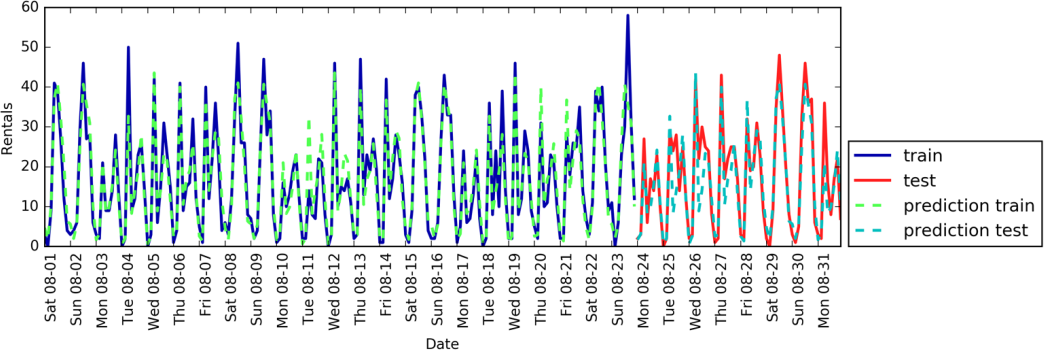
\includegraphics[scale=0.55]{Imagen_Machine/DiaHora2}
	\caption{Predicciones con un bosque aleatorio utilizando las características día de la semana y hora}
	\label{DiaHora2}
\end{figure}


Ahora tenemos un modelo que captura el comportamiento periódico considerando el día de la semana y la hora del día. Tiene un $R^{2}$ de 0.84, y muestra un rendimiento predictivo bastante bueno. 

Lo que este modelo probablemente está aprendiendo es el número promedio de alquileres para cada combinación de día laborable y hora del día a partir de los primeros 23 días de Agosto. Esto en realidad no requiere un modelo complejo como un bosque aleatorio, así que vamos a tratar con un modelo más simple, { \ttfamily  LinearRegression } (ver Figura \ref{DiaHora3}):\\

\begin{lstlisting}%[frame=single]

In[58]:
   
   from sklearn.linear_model import LinearRegression
   eval_on_features(X_hour_week, y, LinearRegression())

Out[58]:

    Test-set R^2: 0.13

\end{lstlisting}



\begin{figure}[h!]
	\centering
	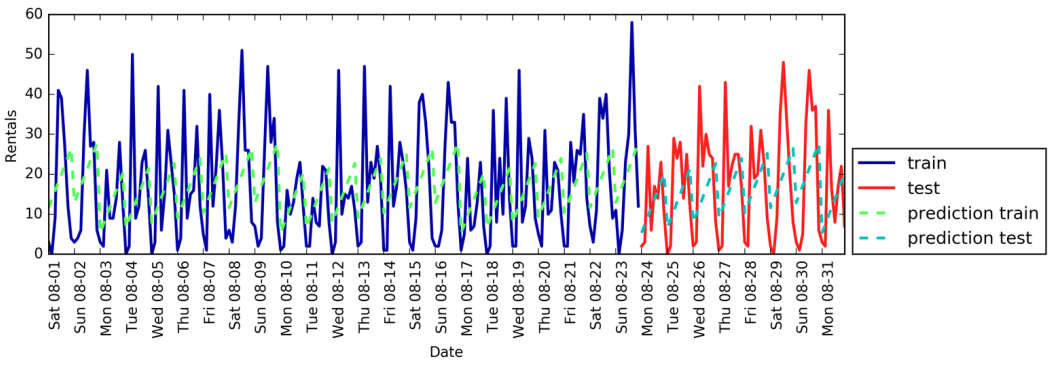
\includegraphics[scale=0.55]{Imagen_Machine/DiaHora3}
	\caption{Predicciones hechas por regresión lineal usando día de semana y hora del día como características}
	\label{DiaHora3}
\end{figure}


El modelo  {\ttfamily LinearRegression}  funciona muy mal o peor, y el patrón periódico parece extraño. 

La razón  para esto es que codificamos día de semana y hora del día usando enteros, el cual es interpretada como variables continuas.  Por lo tanto, el modelo lineal sólo puede aprender una función lineal de la hora del día, y aprendió que más tarde en el día, hay más alquileres. Sin embargo, los patrones son mucho más complejos que eso. Podemos capturar esto interpretando los enteros como variables categóricas, transformándolos usando {\ttfamily One HotEncoder} (ver Figura {DiaHora4}):



\begin{lstlisting}

In[59]:

   enc = OneHotEncoder()
   X_hour_week_onehot = enc.fit_transform(X_hour_week).toarray()
   eval_on_features(X_hour_week_onehot, y, Ridge())

Out[60]:

   Test-set R^2: 0.62

\end{lstlisting}


\begin{figure}[h!]
	\centering
	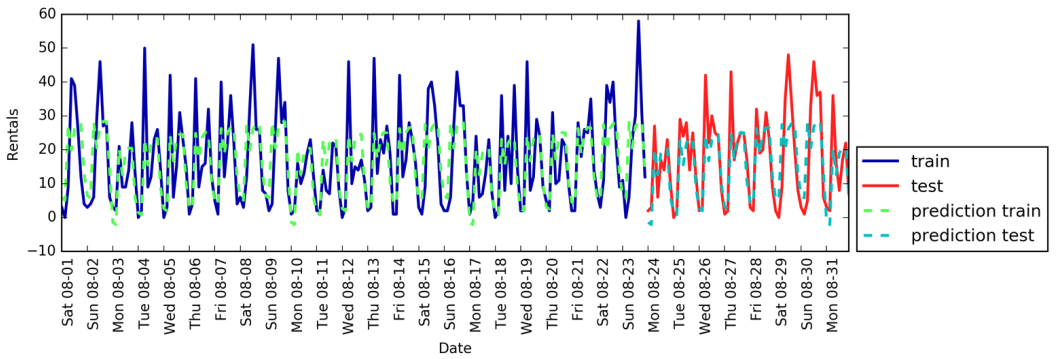
\includegraphics[scale=0.55]{Imagen_Machine/DiaHora4}
	\caption{Predicciones hechas por regresión lineal usando la codificación one-hot del día y del día de la semana}
	\label{DiaHora4}
\end{figure}

Esto nos da un mejor resultado  que la codificación de características como continua. Ahora el modelo lineal aprende un coeficiente para cada día de la semana, y un coeficiente para cada hora del día. Eso significa que el patrón de "{}hora del día"{} se comparte durante todos los días de la semana.\\

% un sin embargo...

Usando  interacción de características, podemos permitir que el modelo aprenda un coeficiente para cada combinación de día y hora del día (ver Figura \ref{DiaHora5}):



\begin{lstlisting}%[frame=single]

In[61]:

   poly_transformer = PolynomialFeatures(degree=2, interaction_only=True,
                                         include_bias=False)
   X_hour_week_onehot_poly = poly_transformer.fit_transform(X_hour_week_onehot)
   lr = Ridge()
   eval_on_features(X_hour_week_onehot_poly, y, lr)

Out[61]:

   Test-set R^2: 0.85

\end{lstlisting}



\begin{figure}[h!]
	\centering
	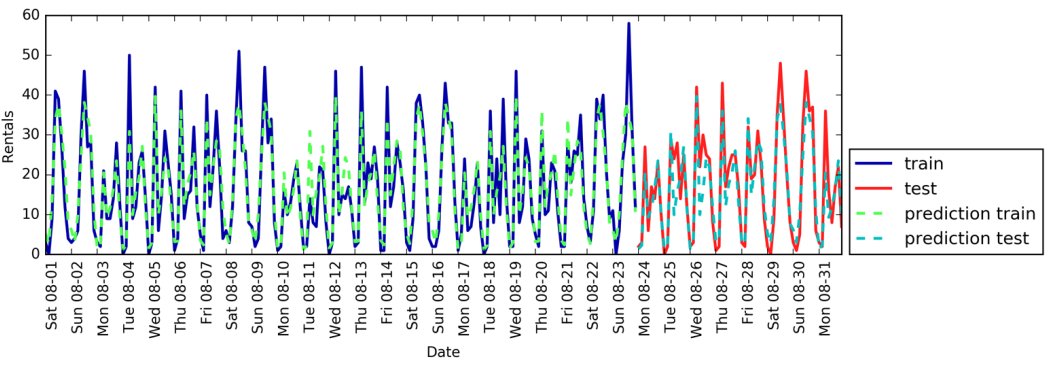
\includegraphics[scale=0.55]{Imagen_Machine/DiaHora5}
	\caption{Predicciones hechas por regresión lineal usando un producto  de las características   día de la semana y  hora del día}
	\label{DiaHora5}
\end{figure}

Esta transformación finalmente produce un modelo que funciona de manera similarmente bien  al  bosque aleatorio. Un gran beneficio de este modelo es que está muy claro lo que es aprendido: un coeficiente para cada día y hora. Podemos simplemente gráficar  los coeficientes aprendidos por el modelo, algo que no sería posible para el bosque aleatorio.\\

  Primero, creamos nombres de características para la hora y día:




\begin{lstlisting}%[frame=single]

In[62]:

   hour = ["%02d:00" % i for i in range(0, 24, 3)]
   day = ["Mon", "Tue", "Wed", "Thu", "Fri", "Sat", "Sun"]
   features = day + hour

\end{lstlisting}


Luego nombramos todas las características de interacción extraídas por {\ttfamily PolynomialFeatures}, usando el método {\ttfamily get\_feature\_names}, y mantenemos sólo las características con coeficientes distinto de cero:\\



\begin{lstlisting}%[frame=single]

In[63]:

   features_poly = poly_transformer.get_feature_names(features)
   features_nonzero = np.array(features_poly)[lr.coef_ != 0]
   coef_nonzero = lr.coef_[lr.coef_ != 0]

\end{lstlisting}



Ahora podemos visualizar los coeficientes aprendidos por el modelo lineal, como se ve en la Figura \ref{ProducHora}:\\

\begin{lstlisting}%[frame=single]

In[64]:

   plt.figure(figsize=(15, 2))
   plt.plot(coef_nonzero, 'o')
   plt.xticks(np.arange(len(coef_nonzero)), features_nonzero, rotation=90)
   plt.xlabel("Feature magnitude")
   plt.ylabel("Feature")

\end{lstlisting}



\begin{figure}[h!]
	\centering
	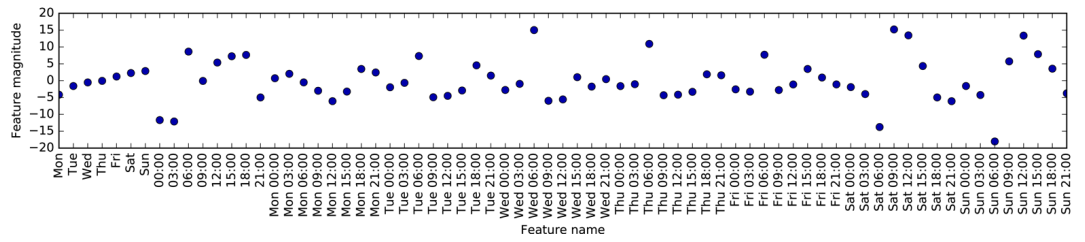
\includegraphics[scale=0.55]{Imagen_Machine/ProducHora}
	\caption{Coeficientes del modelo de regresión lineal utilizando un producto de hora y día}
	\label{ProducHora}
\end{figure}



\section{Resumen y perspectivas}

%  suitable  =   adecuado 

En este capítulo, discutimos cómo tratar los diferentes tipos de datos (en particular, con variables categóricas). Enfatizamos la importancia de representar los datos de una manera que sea adecuada para el algoritmo de aprendizaje automático, por ejemplo, mediante la codificación {\ttfamily one-hot-encoding}.


También discutimos la importancia de la ingeniería de nuevas características, y la posibilidad de utilizar el conocimiento experto en la creación de características derivadas de sus datos. 

En particular, los modelos lineales podrían beneficiarse en gran medida de la generación de nuevas características a través de {\ttfamily binning} y la adición de polinomios e interacciones,mientras que los modelos no lineales más complejos como los bosques aleatorios y las SVMs podrían ser capaces de aprender tareas más complejas sin expandir explícitamente el espacio de características.
En la práctica, las características que se utilizan (y la coincidencia entre las características y el método) es a menudo la pieza más importante para hacer que un enfoque de aprendizaje automático funcione bien.
 

Ahora que usted tiene una buena idea de cómo representar los datos de una manera apropiada y qué algoritmo utilizar para la tarea, el próximo capítulo se centrará en la evaluación del rendimiento de los modelos de aprendizaje automático y la selección de la configuración de parámetros adecuados.

%%%%%%%%%%%                 %%%%%%%%%%%%%%%%%%%%%%%%%%